\documentclass[aspectratio=169,11pt]{beamer}
\geometry{paperwidth=13.333in,paperheight=7.5in}

\usepackage{iftex}
\ifPDFTeX
  \usepackage[T1]{fontenc}
  \usepackage[utf8]{inputenc}
\else
  \usepackage{fontspec}
  \setsansfont{Carlito}[
    Path=../.tools/fonts/,
    UprightFont=*-Regular.ttf,
    BoldFont=*-Bold.ttf,
    ItalicFont=*-Italic.ttf,
    BoldItalicFont=*-BoldItalic.ttf
  ]
  \setmainfont{Carlito}[
    Path=../.tools/fonts/,
    UprightFont=*-Regular.ttf,
    BoldFont=*-Bold.ttf,
    ItalicFont=*-Italic.ttf,
    BoldItalicFont=*-BoldItalic.ttf
  ]
  \setmonofont{DejaVu Sans Mono}[Scale=MatchLowercase]
\fi
\usepackage{booktabs}
\usepackage{array}
\usepackage{pgfgantt}
\usepackage{sff_theme}

\title[Rapid Microstructure Prediction]{Rapid Microstructure Prediction in Laser Powder Bed Fusion\\ Using Bayesian Updating of Eagar--Tsai Model}
\subtitle{}
\author[Swartz, Hanagan, Vela, Sarıtürk, Arróyave]{Kyle Swartz, James Hanagan, Brent Vela, Doğuhan Sarıtürk, Raymundo Arróyave}
\institute[TAMU]{Department of Materials Science and Engineering, Texas A\&M University}
\date{August 3, 2026}

\begin{document}

\begin{frame}
  \titlepage
\end{frame}

\begin{frame}{Core Thesis}
  \begin{columns}[T,onlytextwidth]
    \begin{column}{0.32\textwidth}
      \begin{block}{Composition}
        \centering
        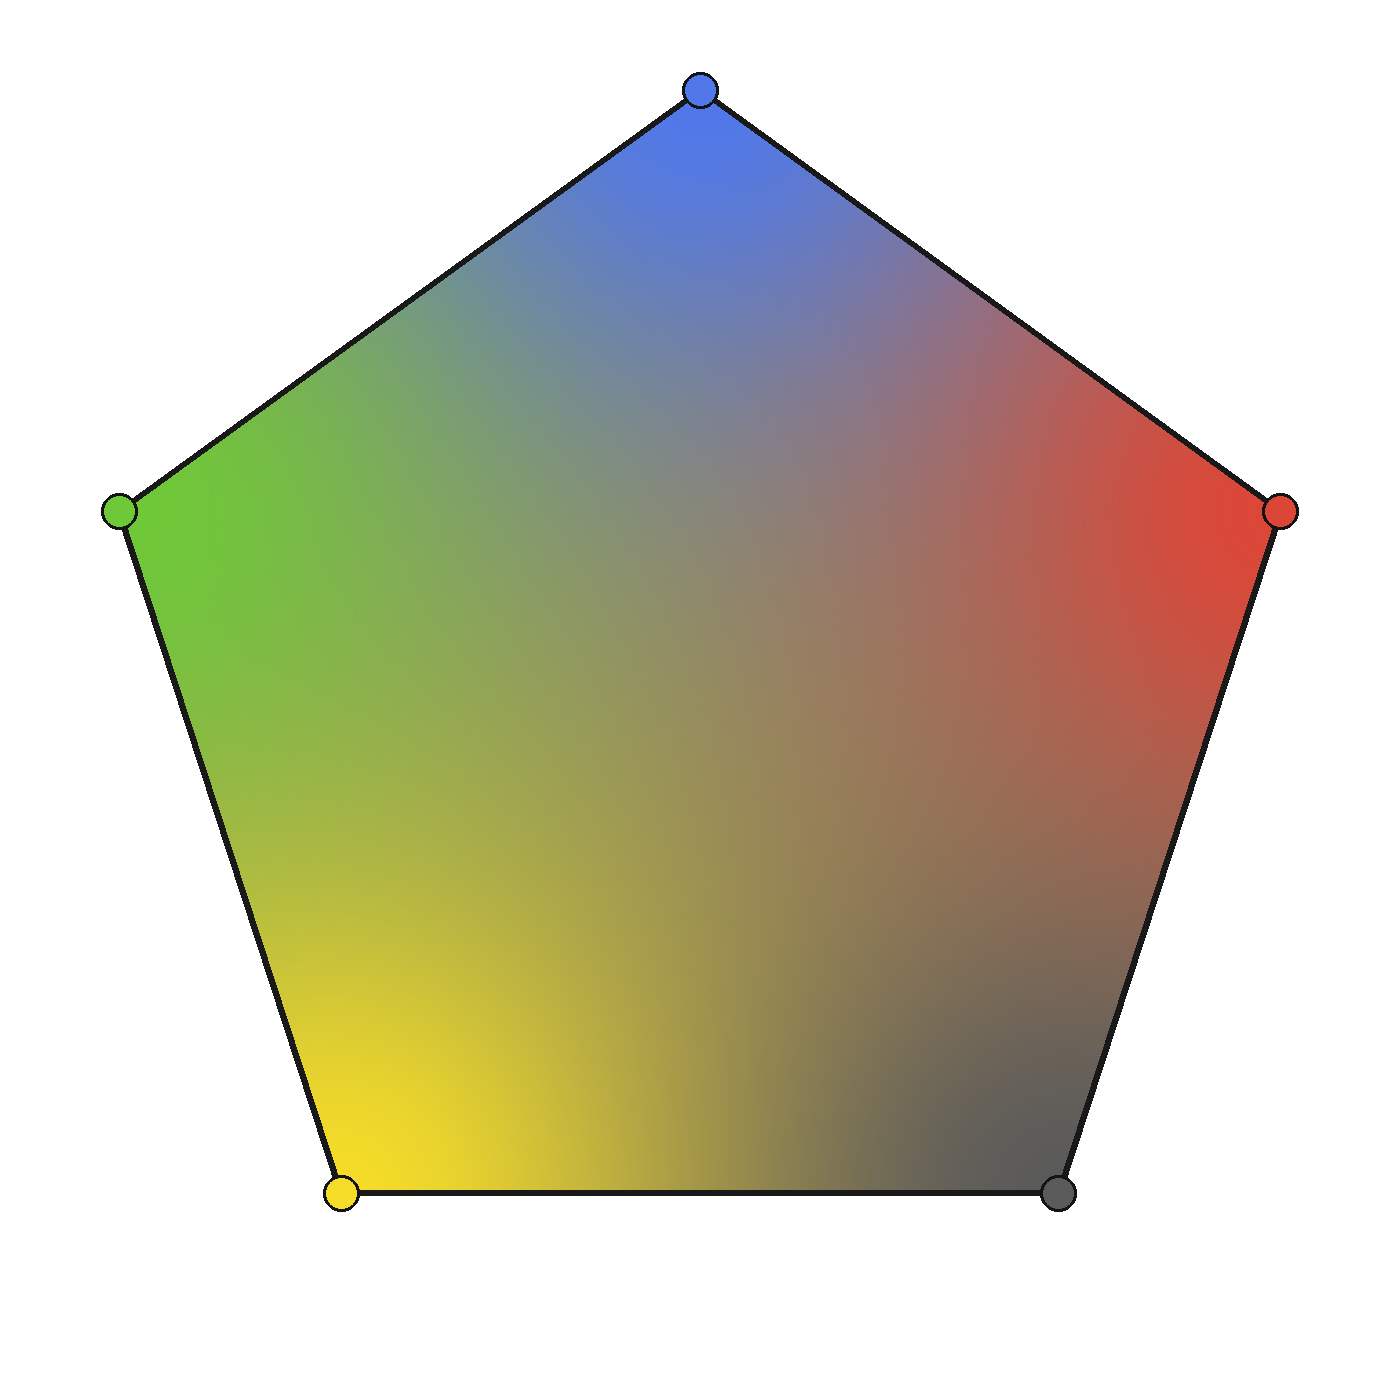
\includegraphics[width=\linewidth,height=0.28\textheight,keepaspectratio]{figures/affine_projection_nimplex_nb_cr_v_w_zr_20pct_pentagon_clean.png}

        \vspace{0.25em}
        \begin{itemize}
          \item A 5-element affine projection represents the accessible composition simplex.
          \item Interior coloring encodes local element content across the design space.
          \item Bayesian updates narrow the search to feasible LPBF compositions.
        \end{itemize}
      \end{block}
    \end{column}
    \begin{column}{0.32\textwidth}
      \begin{block}{Solidification Condition}
        \centering
        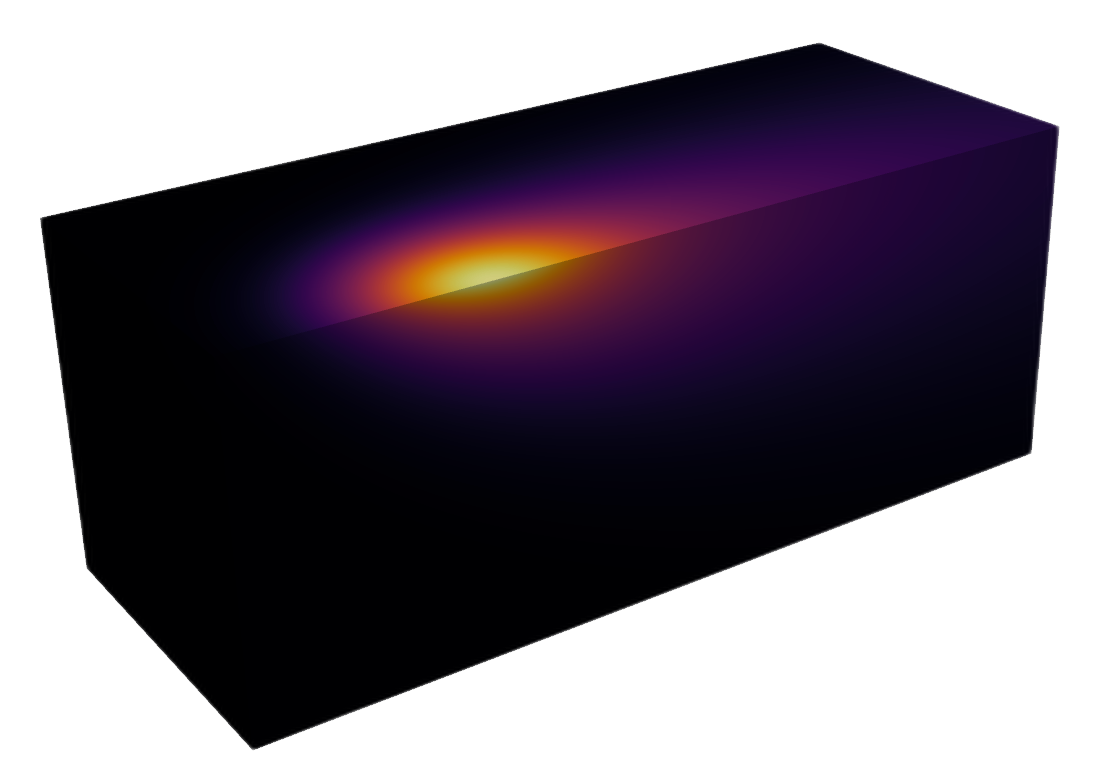
\includegraphics[width=\linewidth,height=0.27\textheight,keepaspectratio]{figures/et_solidification_condition.png}

        \vspace{0.2em}
        \begin{itemize}
          \item Real `eagar-tsai` VTI render with the symmetry-plane melt-pool slice.
          \item Process inputs set the thermal gradient, cooling rate, and pool geometry.
        \end{itemize}
      \end{block}
    \end{column}
    \begin{column}{0.32\textwidth}
      \begin{alertblock}{Solidified Microstructure}
        \begin{itemize}
          \item Microstructure emerges from the coupling of chemistry and thermal history.
          \item Predicted G/R conditions map to expected grain morphology and phase selection.
          \item The workflow targets rapid microstructure prediction from composition to final structure.
        \end{itemize}
      \end{alertblock}
    \end{column}
  \end{columns}
\end{frame}

\begin{frame}{Motivation and Constraints}
  \vspace{-0.35em}
  \begin{columns}[T,onlytextwidth]
    \begin{column}{0.49\textwidth}
      {\fontsize{20}{24}\selectfont\textcolor{sffblue}{\textbf{The design target is microstructure}}\par}
      \vspace{0.35em}
      \begin{itemize}
        \item LPBF alloy design couples composition, laser power, scan speed, and cooling history.
        \item Grain morphology and phase selection respond to local thermal gradients, $G$, and solidification rates, $R$.
        \item Screening must move quickly from process inputs to a microstructure-relevant prediction.
      \end{itemize}

      \vspace{0.25em}
      \begin{alertblock}{Constraint}
        Eagar--Tsai is fast enough for high-throughput screening, but its simplified thermal physics must be corrected before it can be trusted for microstructure decisions.
      \end{alertblock}
    \end{column}
    \begin{column}{0.47\textwidth}
      \centering
      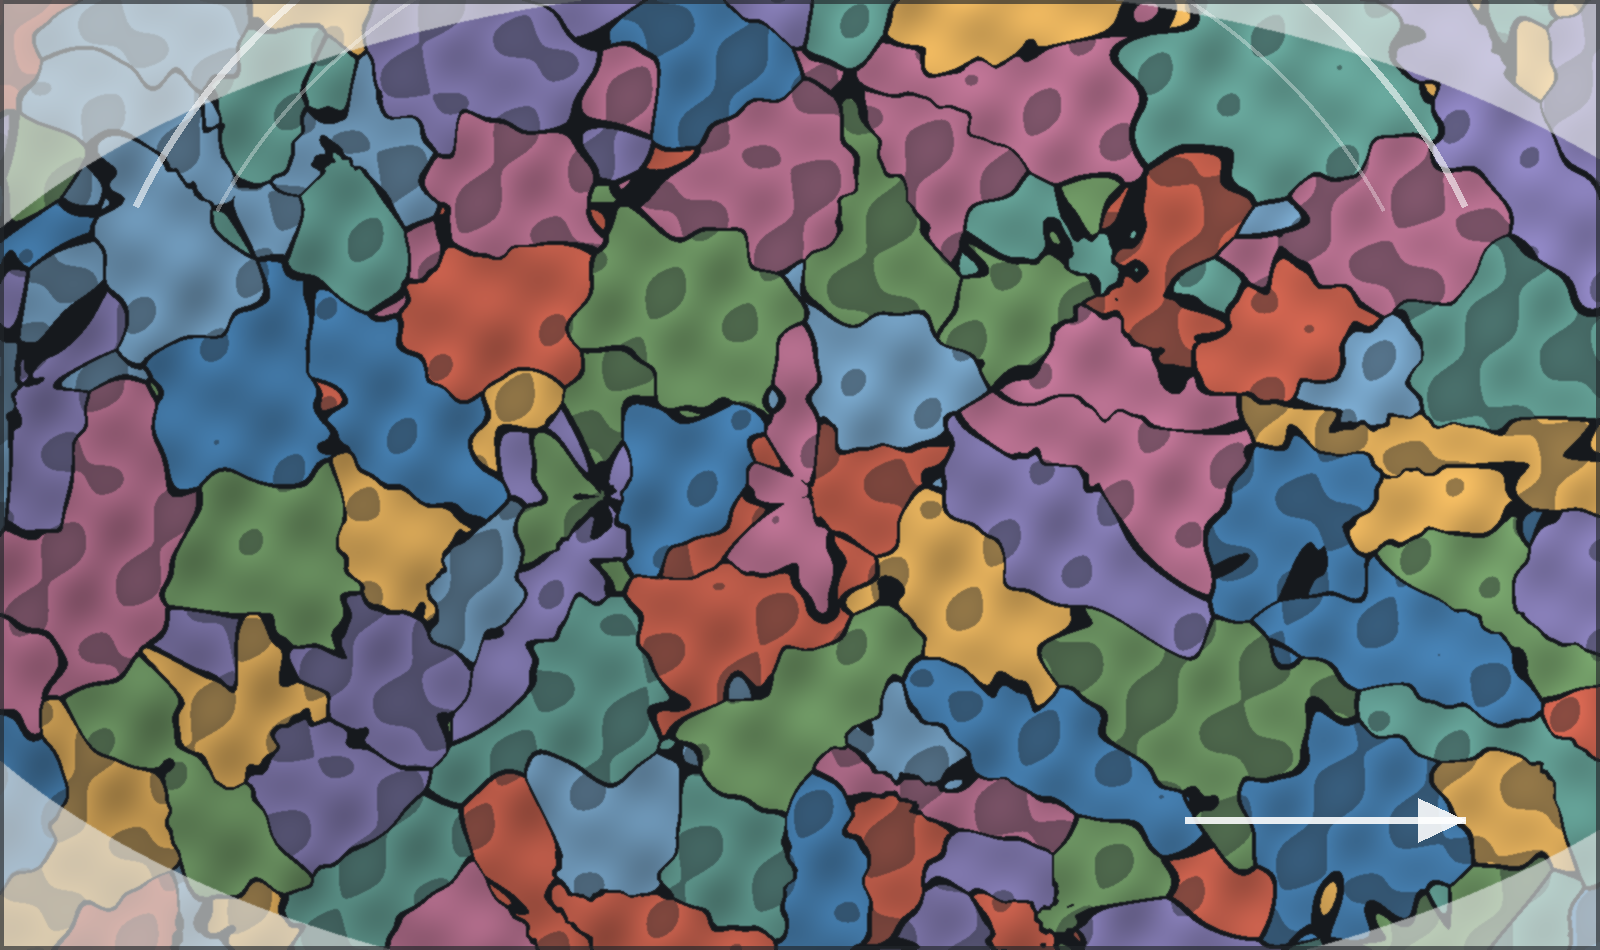
\includegraphics[width=\linewidth,height=0.55\textheight,keepaspectratio]{../beamer/figures/phase_field_microstructure_proxy.png}

      \vspace{0.2em}
      {\fontsize{14}{17}\selectfont Illustrative phase-field style proxy: the model must connect melt-pool thermal history to grain morphology and phase contrast.\par}

      \vspace{0.25em}
      {\fontsize{13}{16}\selectfont\textcolor{neutralmid}{Key limits: temperature-invariant properties, analytical melt-pool assumptions, and lower fidelity than FEM.}\par}
    \end{column}
  \end{columns}
\end{frame}

\begin{frame}{Cellular Automata Solidification Modes}
  \vspace{-0.45em}
  \begin{columns}[T,onlytextwidth]
    \begin{column}{0.31\textwidth}
      \centering
      {\fontsize{18}{22}\selectfont\textcolor{sffblue}{\textbf{Dendritic}}\par}
      \vspace{0.2em}
      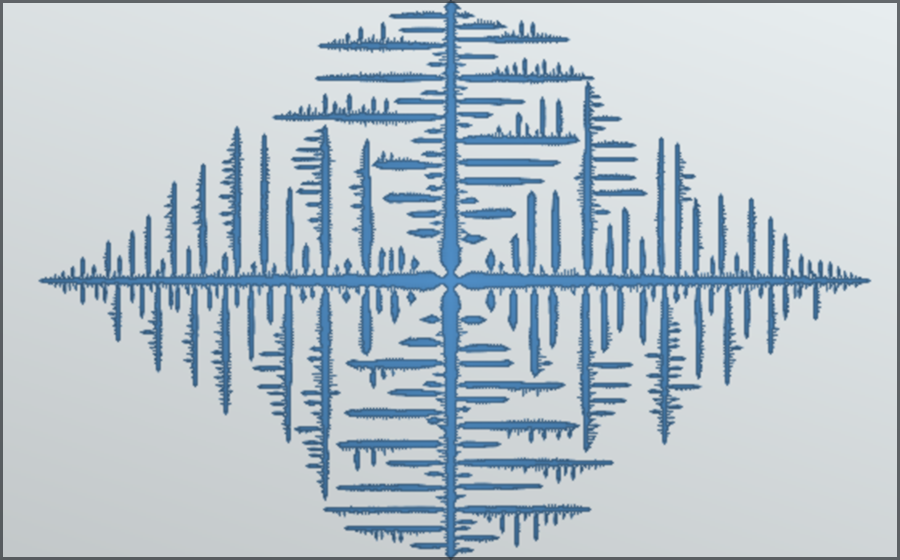
\includegraphics[width=\linewidth,height=0.40\textheight,keepaspectratio]{../beamer/figures/ca_modes/ca_dendritic.png}

      \vspace{0.2em}
      {\fontsize{13}{16}\selectfont Branching growth when interface perturbations are amplified by undercooling and solute rejection.\par}
    \end{column}
    \begin{column}{0.31\textwidth}
      \centering
      {\fontsize{18}{22}\selectfont\textcolor{sffblue}{\textbf{Columnar}}\par}
      \vspace{0.2em}
      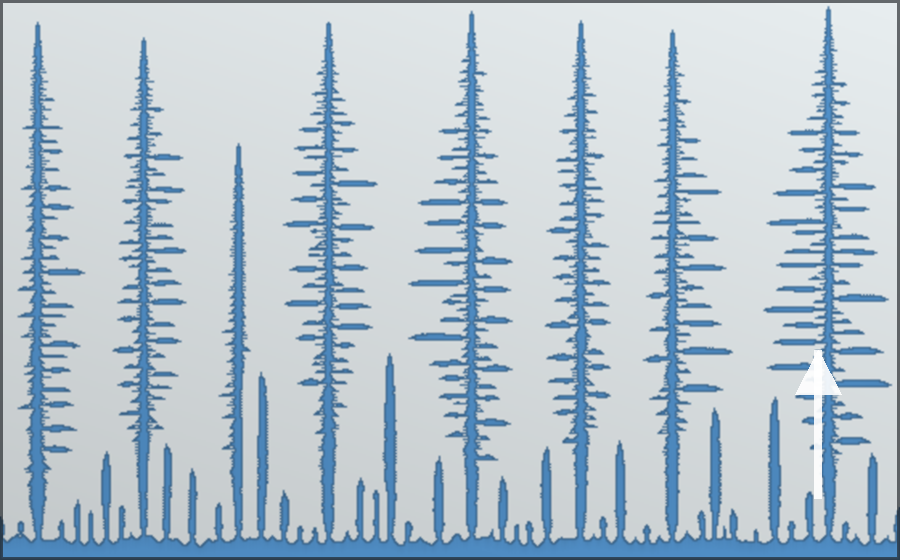
\includegraphics[width=\linewidth,height=0.40\textheight,keepaspectratio]{../beamer/figures/ca_modes/ca_columnar_dendritic.png}

      \vspace{0.2em}
      {\fontsize{13}{16}\selectfont Competing primary trunks aligned with heat flow select $\lambda_1$; sidebranching sets $\lambda_2$.\par}
    \end{column}
    \begin{column}{0.31\textwidth}
      \centering
      {\fontsize{18}{22}\selectfont\textcolor{sffblue}{\textbf{Planar}}\par}
      \vspace{0.2em}
      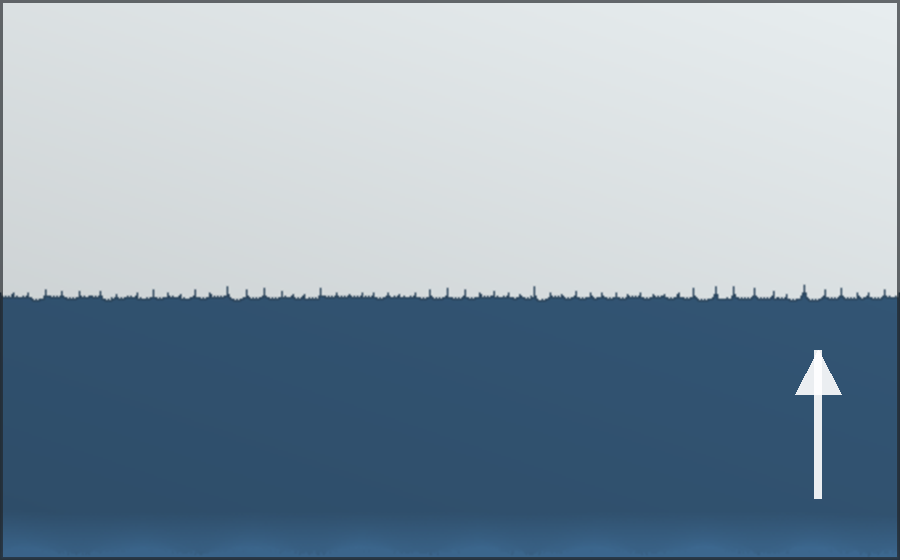
\includegraphics[width=\linewidth,height=0.40\textheight,keepaspectratio]{../beamer/figures/ca_modes/ca_planar.png}

      \vspace{0.2em}
      {\fontsize{13}{16}\selectfont A stable solid--liquid front advances when the thermal gradient suppresses morphological instability.\par}
    \end{column}
  \end{columns}

  \vspace{0.25em}
  \begin{alertblock}{Use in this workflow}
    Eagar--Tsai supplies fast local $G$ and $R$ fields; Bayesian correction should make those fields reliable enough to classify morphology regime.
  \end{alertblock}
\end{frame}

\begin{frame}{KGT Solidification Theory}
  \vspace{-0.35em}
  \begin{columns}[T,onlytextwidth]
    \begin{column}{0.52\textwidth}
      \begin{block}{Kurz--Giovanola--Trivedi framework}
        \begin{itemize}
          \item KGT links dendrite-tip operating state to local thermal gradient, $G$, and interface growth rate, $R$.
          \item The dendrite tip is approximated locally as a paraboloid with radius of curvature $\rho$.
          \item Tip selection then relates $\rho$ to $R$ and alloy transport and capillarity properties.
        \end{itemize}
      \end{block}

      \vspace{0.25em}
      \begin{alertblock}{Why it matters here}
        ET supplies local $G$ and $R$ along the solidification front. KGT uses those fields, together with material properties, to connect melt-pool conditions to dendrite-tip size and morphology selection.
      \end{alertblock}

      \vspace{0.1em}
      \centering
      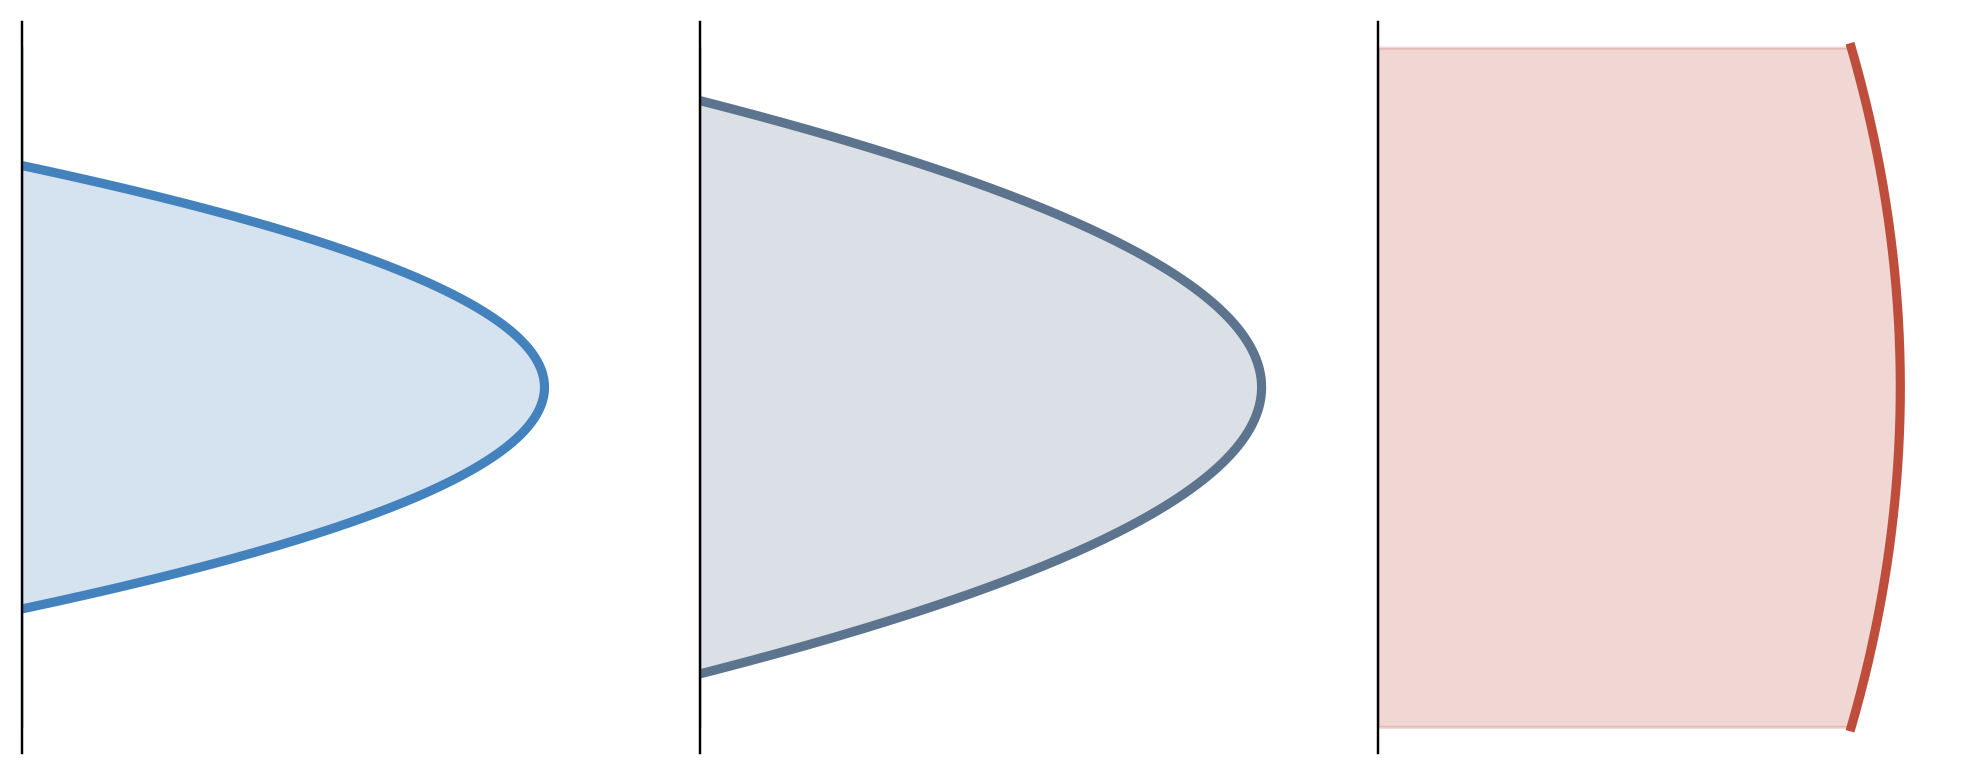
\includegraphics[width=\linewidth,height=0.34\textheight,keepaspectratio]{../beamer/figures/kgt_tip_radii.png}
    \end{column}
    \begin{column}{0.44\textwidth}
      {\fontsize{19}{23}\selectfont\textcolor{sffblue}{\textbf{Tip relations}}\par}
      \vspace{0.35em}
      {\fontsize{15}{18}\selectfont
      \[
      z = \frac{x^2 + y^2}{2\rho}
      \]
      \[
      Pe = \frac{\rho R}{2D_l}
      \]
      \[
      \sigma^* = \frac{2D_l d_0}{\rho^2 R}
      \]
      \[
      \rho = \left(\frac{2D_l d_0}{\sigma^* R}\right)^{1/2}
      \]
      \[
      d_0 \approx \frac{\Gamma}{|m|\,C_0(1-k)/k}
      \]
      }

      \vspace{0.35em}
      \begin{itemize}
        \item $D_l$: liquid diffusivity, $\Gamma$: Gibbs--Thomson coefficient, $m$: liquidus slope.
        \item $C_0$: nominal composition, $k$: partition coefficient, $\sigma^*$: tip-selection parameter.
        \item Higher $R$ gives a smaller selected tip radius $\rho$ for fixed material properties.
      \end{itemize}

      \vspace{0.2em}
      {\fontsize{13}{16}\selectfont\textcolor{neutralmid}{In this workflow, $G$ determines the imposed thermal field and morphology stability, while $R$ enters directly into the selected paraboloid tip radius.}\par}
    \end{column}
  \end{columns}
\end{frame}

\begin{frame}{Eagar--Tsai Model Foundation}
  \vspace{-0.55em}
  \begin{columns}[T,onlytextwidth]
    \begin{column}{0.49\textwidth}
      \centering
      {\fontsize{22}{26}\selectfont\textcolor{sffblue}{\textbf{Original Eagar--Tsai Paper}}\par}
      \vspace{0.28em}

      {\fontsize{15}{18}\selectfont Transient Gaussian moving heat source}
      \vspace{0.35em}

      \begin{minipage}[t][0.64\textheight][t]{\linewidth}
        \begin{tikzpicture}[x=\linewidth,y=1cm]
          \node[anchor=north east,inner sep=0pt] at (1.0,2.4) {
            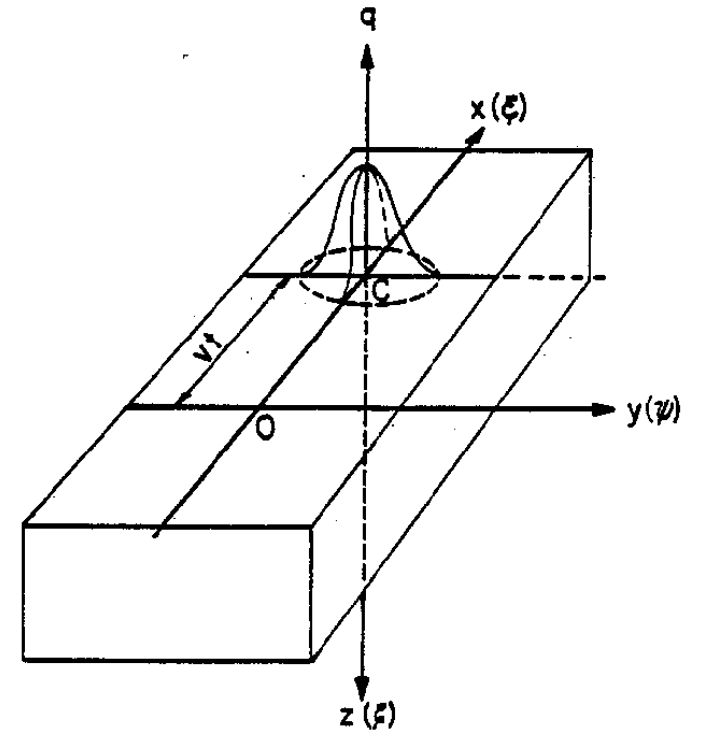
\includegraphics[width=0.50\linewidth]{../beamer/figures/eagar_tsai_og_figure.png}
          };
          \node[anchor=west,inner sep=0pt,text width=0.98\linewidth] at (0.0,3.05) {
            {\fontsize{15}{18}\selectfont
            \(\displaystyle
            \begin{aligned}
            T - T_0
            &= \frac{1}{2}\int_{0}^{t} dT_i \\
            &= \frac{q}{\pi\rho C_p\sqrt{4\pi\alpha}}
            \int_{0}^{t}
            \frac{(t-t')^{-1/2}}
                 {2\alpha(t-t')+\sigma^2} \\
            &\times
            \exp\Bigg[
            -\frac{(x-vt')^2+y^2}{4\alpha(t-t')+2\sigma^2}
            -\frac{z^2}{4\alpha(t-t')}
            \Bigg]\,dt'
            \end{aligned}
            \)
            }
          };
          \node[
            overlay,
            anchor=north west,
            inner sep=0pt,
            align=left,
            text width=0.48\linewidth
          ] at (0.01,-1.35) {
            {\fontsize{18}{22}\selectfont
            {\fontsize{22}{26}\selectfont\textcolor{sffblue}{\textbf{Inputs}}}\par
            \textbf{Process:} $P$, $v$, $d_b$, $A$\par
            \textbf{Material:} $T_L$, $k_L$, $\rho_0$, $C_p$
            }
          };
          \path (0,0) rectangle (1,4.25);
        \end{tikzpicture}
        \vfill
        {\fontsize{12.5}{15}\selectfont Eagar, T. W., \& Tsai, N. S. (1983). Temperature fields produced by traveling distributed heat sources. \textit{Welding Journal, 62}(12), 346--355.}
      \end{minipage}
    \end{column}
    \begin{column}{0.02\textwidth}
      \centering
      \vspace{-0.15em}
      \rule{0.5pt}{0.80\textheight}
    \end{column}
    \begin{column}{0.49\textwidth}
      \centering
      {\fontsize{22}{26}\selectfont\textcolor{sffblue}{\textbf{Refactored Eagar--Tsai Model}}\par}
      \vspace{0.18em}
      {\fontsize{15}{18}\selectfont Python library implementation with compiled-C speedup\par}
      \vspace{0.25em}

      \begin{tikzpicture}[x=\linewidth,y=1cm]
        \node[anchor=north,inner sep=0pt] at (0.37,-0.72) {
          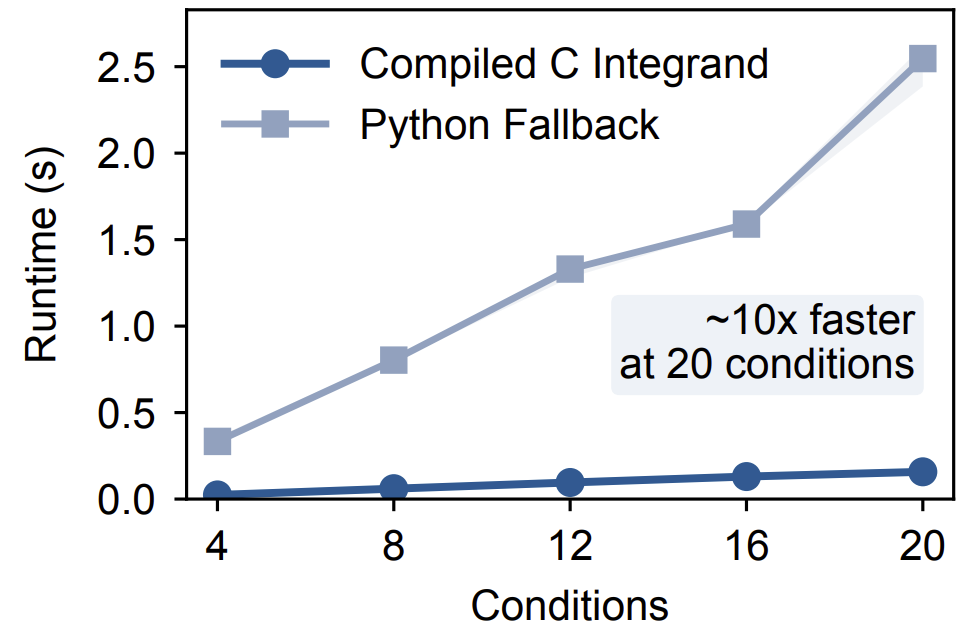
\includegraphics[width=0.66\linewidth]{../beamer/figures/dogu_figure_f.png}
        };
        \node[anchor=center,inner sep=0pt] at (0.82,-3.50) {
          
\includegraphics[width=0.23\linewidth]{../beamer/figures/logo.png}
        };
        \path (0,-4.45) rectangle (1,0);
      \end{tikzpicture}
      \vspace{0.05em}
      {\raggedright
      \begin{itemize}
        \item Separates melt-pool prediction, printability maps, 2D heatmap generation, and 3D temperature-field export into reusable steps.
        \item Compiled C integrand removes Python overhead inside QUADPACK for faster parameter sweeps.
      \end{itemize}
      }
    \end{column}
  \end{columns}
\end{frame}

\begin{frame}{ET Thermal Cross Sections}
  \begin{columns}[T,onlytextwidth]
    \begin{column}{0.49\textwidth}
      \centering
      \begin{minipage}[t][0.68\textheight][c]{\linewidth}
        \centering
        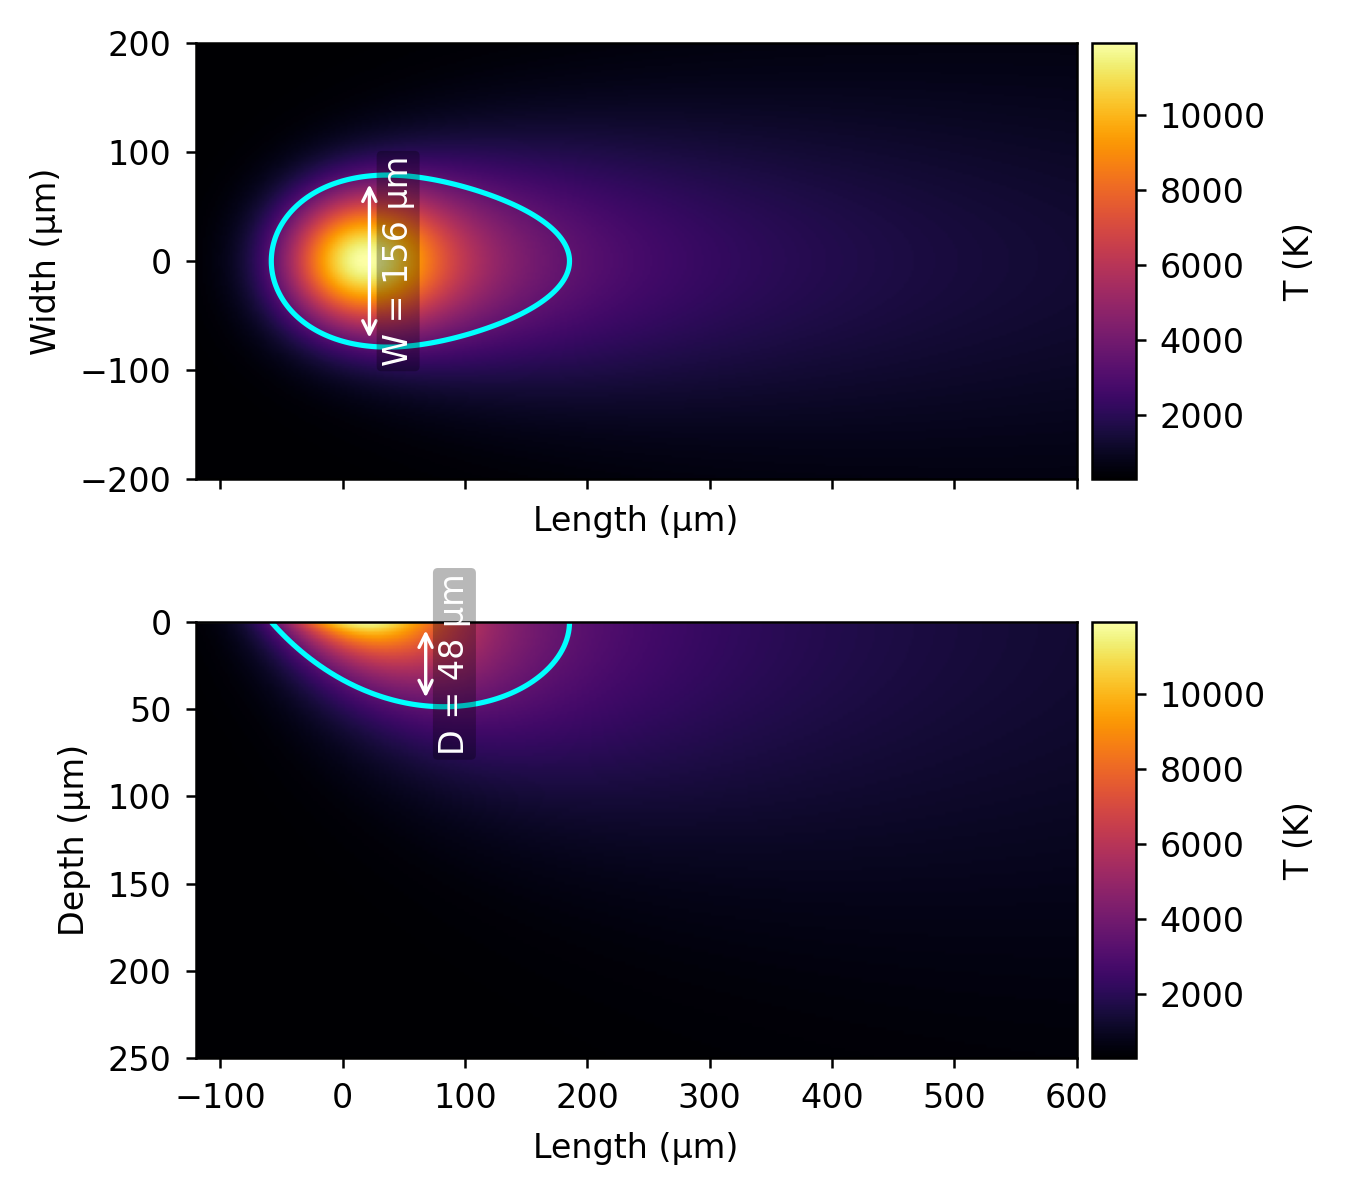
\includegraphics[width=\linewidth,height=0.68\textheight,keepaspectratio]{../beamer/figures/250_0.5/temperature_field_alloy0_250_0.5.png}
      \end{minipage}

      \vspace{0.25em}
      {\fontsize{15}{18}\selectfont Temperature heatmap for Hf$_2$Mo$_2$Ta$_{48}$W$_{48}$ (at.\%), $P = 250$ W and $V = 0.5$ m/s. Top: $z = 0$ surface. Bottom: $y = 0$ cross section.}
    \end{column}
    \begin{column}{0.49\textwidth}
      \centering
      \begin{minipage}[t][0.68\textheight][c]{\linewidth}
        \centering
        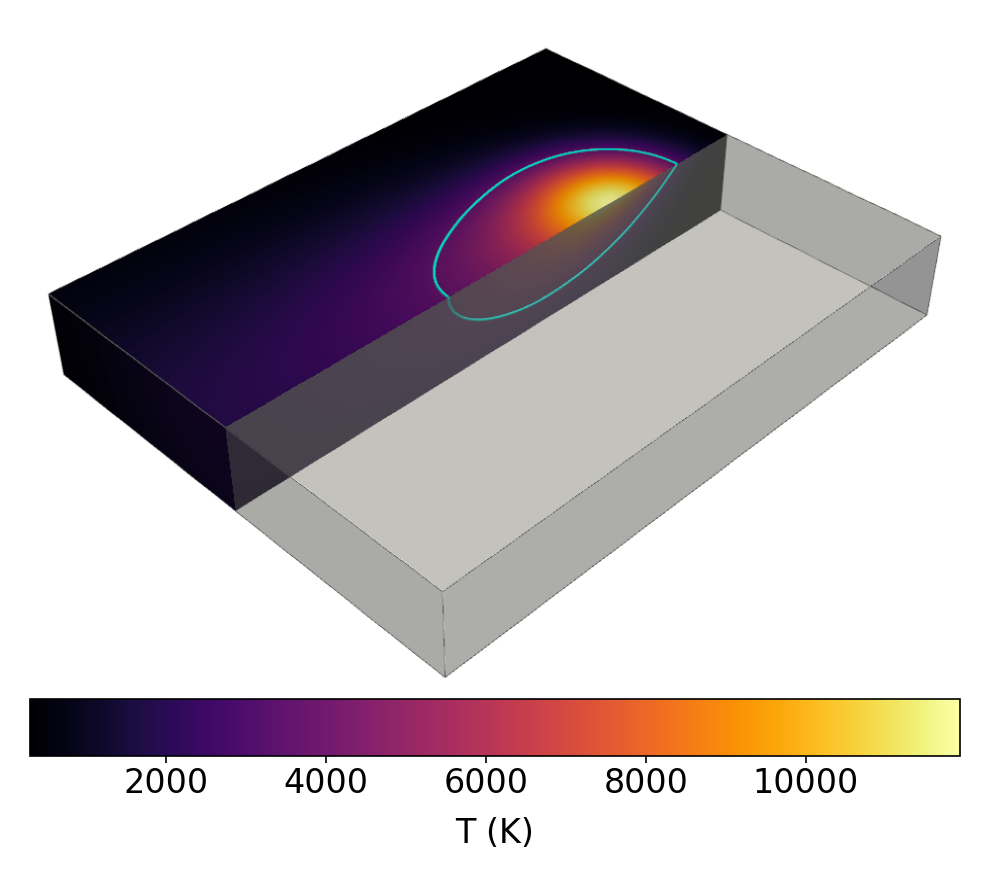
\includegraphics[width=\linewidth,height=0.68\textheight,keepaspectratio]{../beamer/figures/250_0.5/ET_3D_temperature_alloy0_250_0.5.png}
      \end{minipage}

      \vspace{0.25em}
      {\fontsize{15}{18}\selectfont 3D view of the ET melt pool for the same alloy and process condition.}
    \end{column}
  \end{columns}
\end{frame}

\begin{frame}{ET Thermal Gradient and Solidification Rate}
  \begin{columns}[T,onlytextwidth]
    \begin{column}{0.45\textwidth}
      \centering
      \begin{minipage}[t][0.58\textheight][c]{\linewidth}
        \centering
        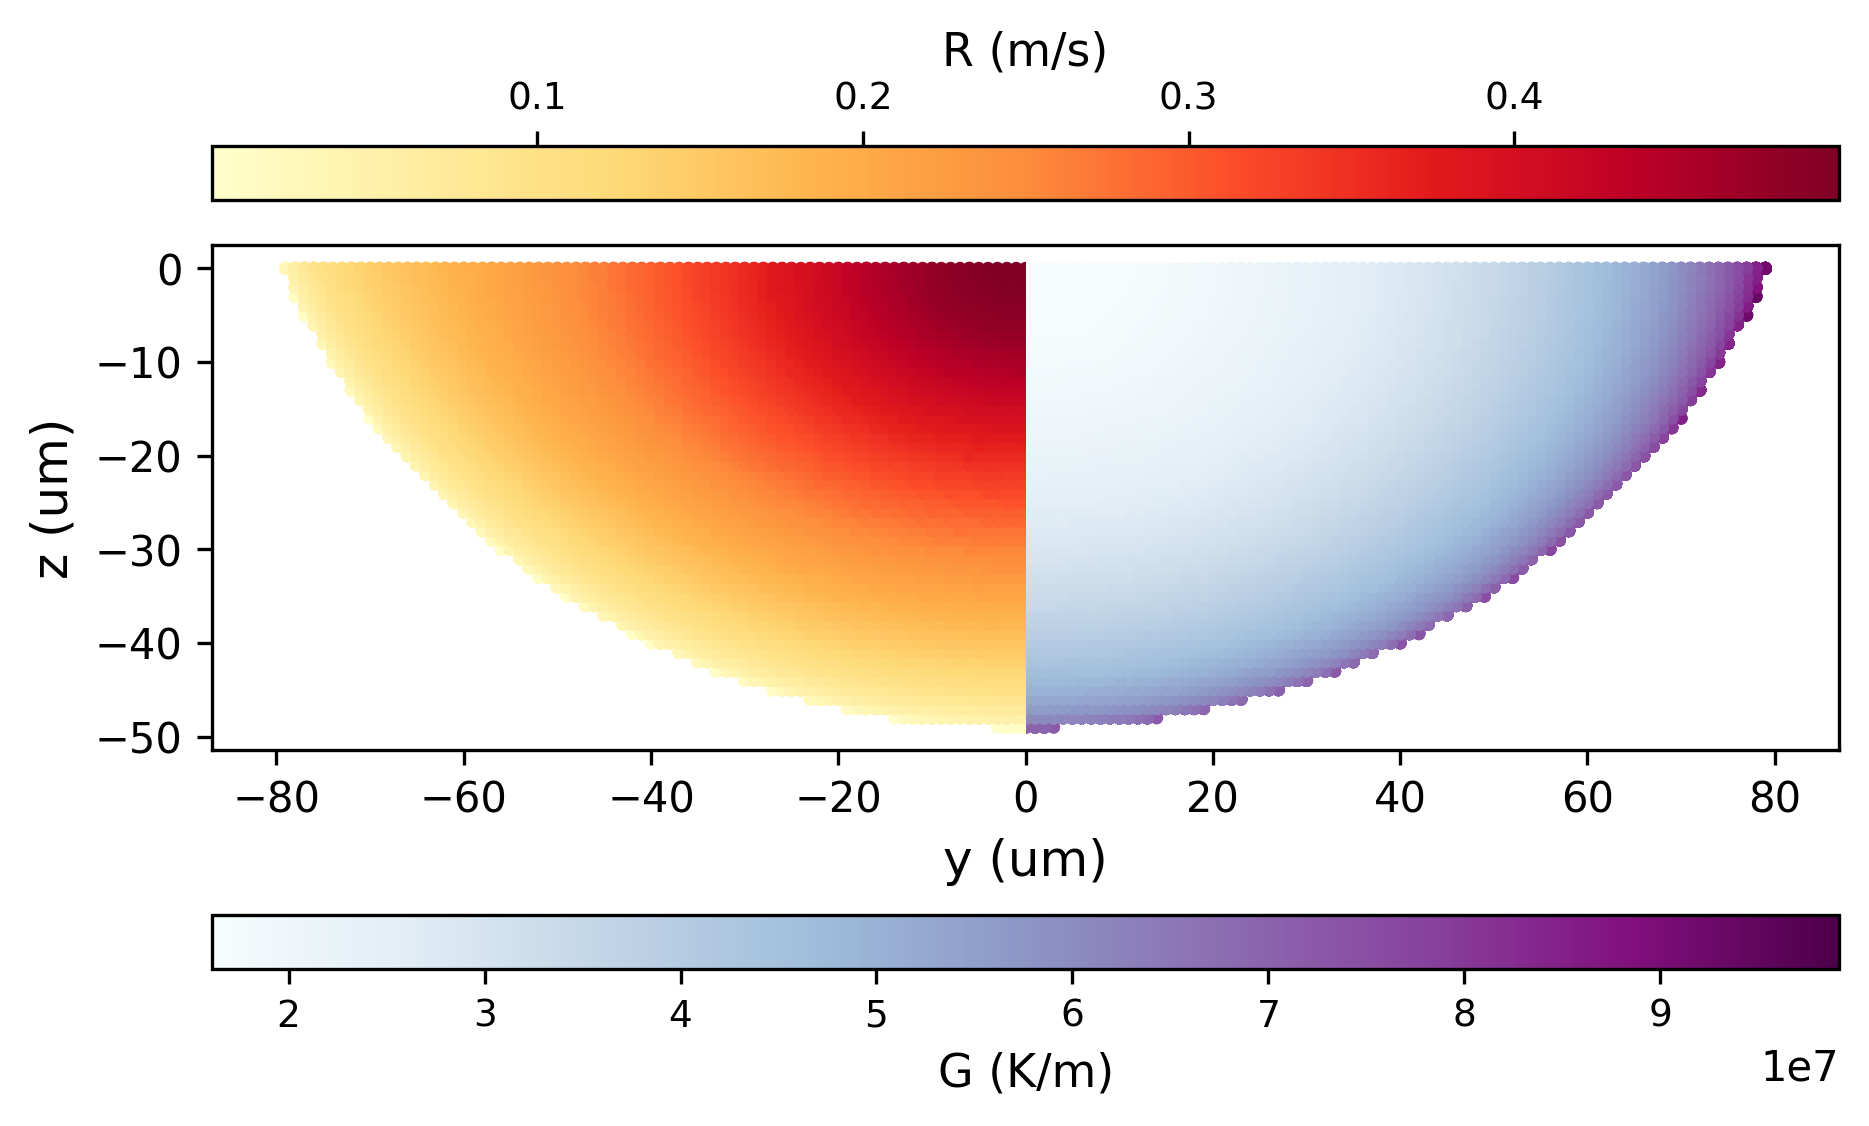
\includegraphics[width=\linewidth,height=0.58\textheight,keepaspectratio]{../beamer/figures/250_0.5/projected_GR_alloy0_250_0.5.png}
      \end{minipage}

      \vspace{0.25em}
      {\fontsize{15}{18}\selectfont Projection of $G$ and $R$ along the solidification front onto a $yz$ slice for Hf$_2$Mo$_2$Ta$_{48}$W$_{48}$ (at.\%), $P = 250$ W and $V = 0.5$ m/s.}
    \end{column}
    \begin{column}{0.08\textwidth}
      \centering
      \vspace{0.25\textheight}
      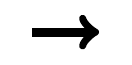
\begin{tikzpicture}
        \draw[->,line width=3.2pt,draw=black] (0,0) -- (0.85,0);
      \end{tikzpicture}
    \end{column}
    \begin{column}{0.45\textwidth}
      \centering
      \begin{minipage}[t][0.58\textheight][c]{\linewidth}
        \centering
        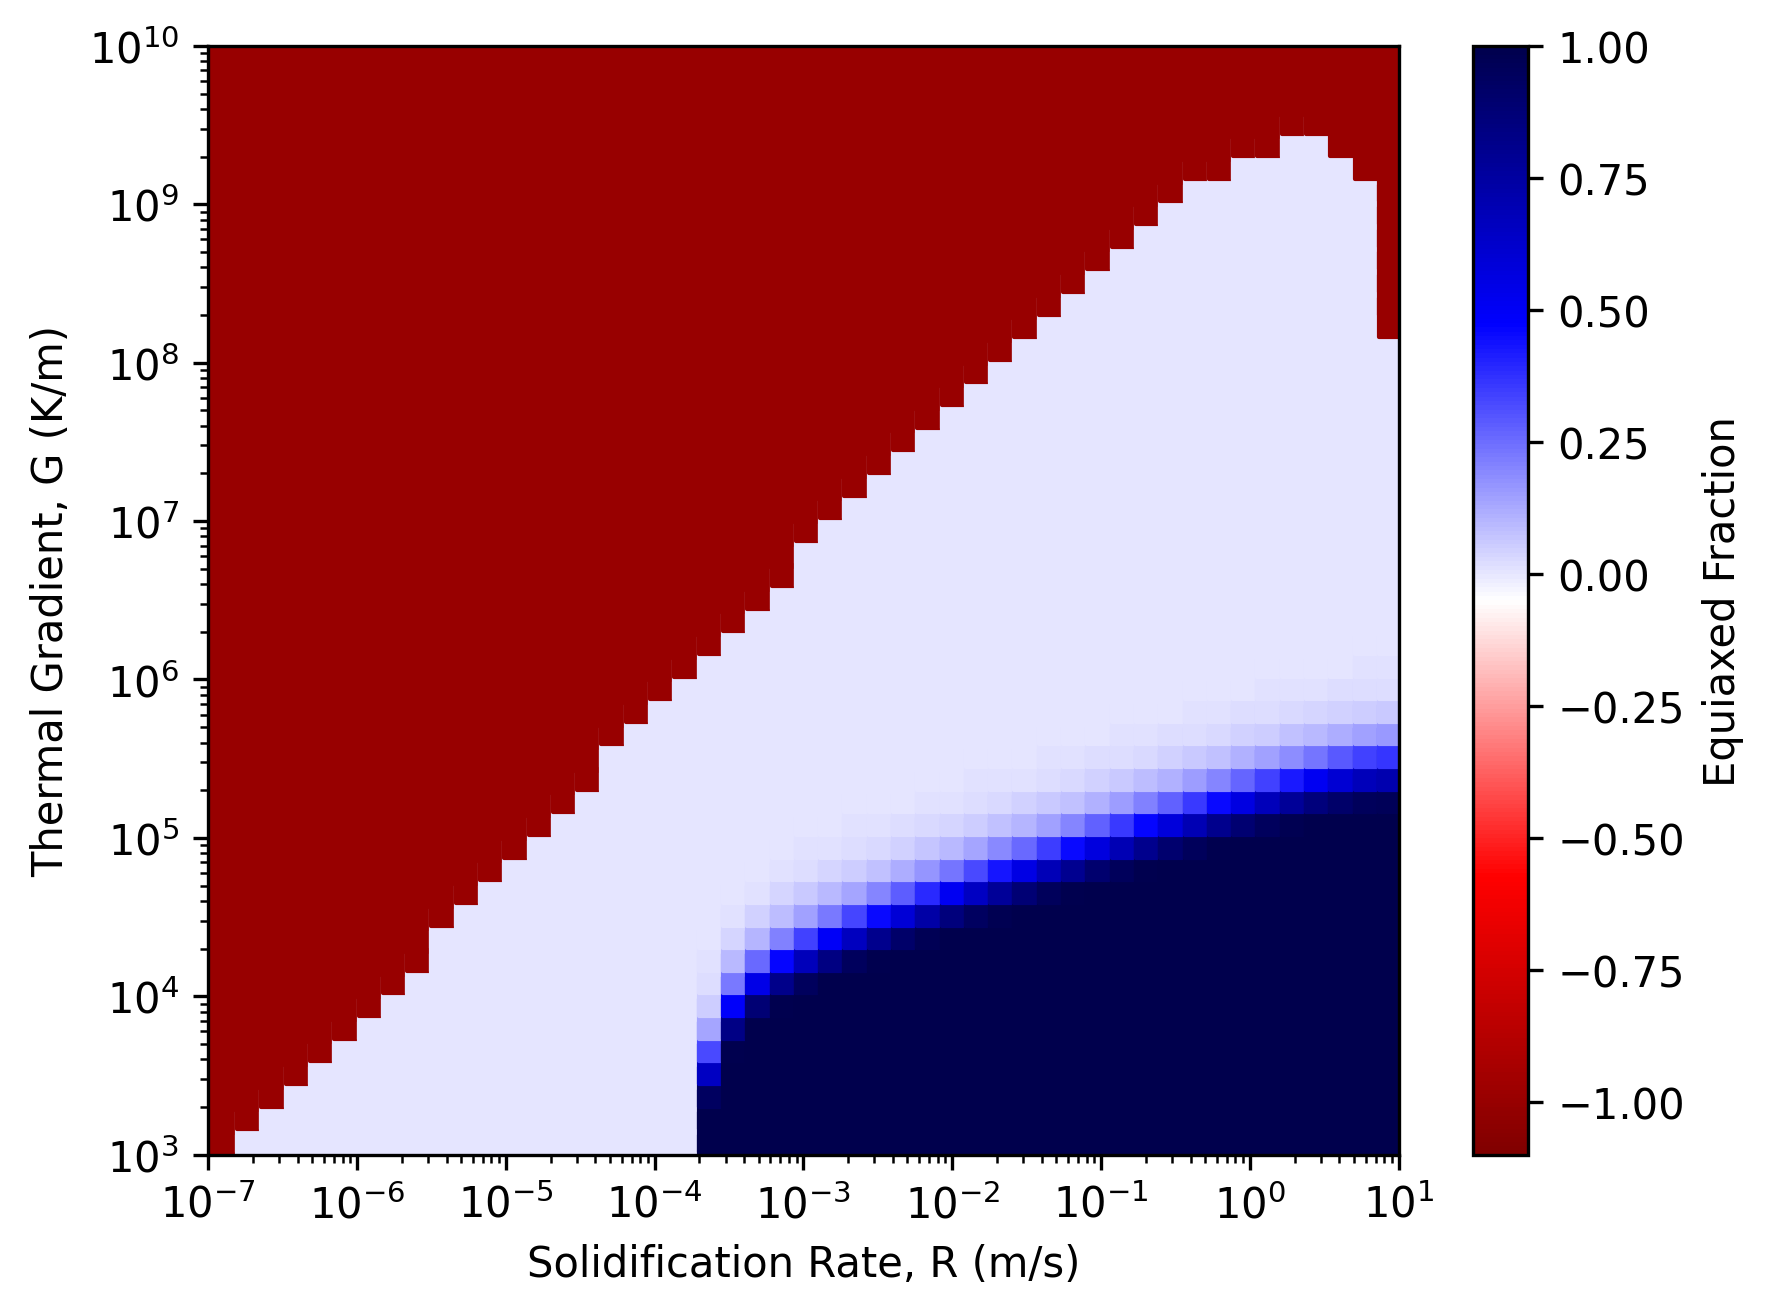
\includegraphics[width=\linewidth,height=0.58\textheight,keepaspectratio]{../beamer/figures/TCAM/GR_map_alloy0_250_0.5.png}
      \end{minipage}

      \vspace{0.25em}
      {\fontsize{15}{18}\selectfont GR Map calculated with Thermo-Calc CET Property Model for Hf$_2$Mo$_2$Ta$_{48}$W$_{48}$ (at.\%), $P = 250$ W and $V = 0.5$ m/s.}
    \end{column}
  \end{columns}
\end{frame}

\begin{frame}{ET Microstructure Classification}
  \begin{columns}[T,onlytextwidth]
    \begin{column}{0.45\textwidth}
      \centering
      \begin{minipage}[t][0.58\textheight][c]{\linewidth}
        \centering
        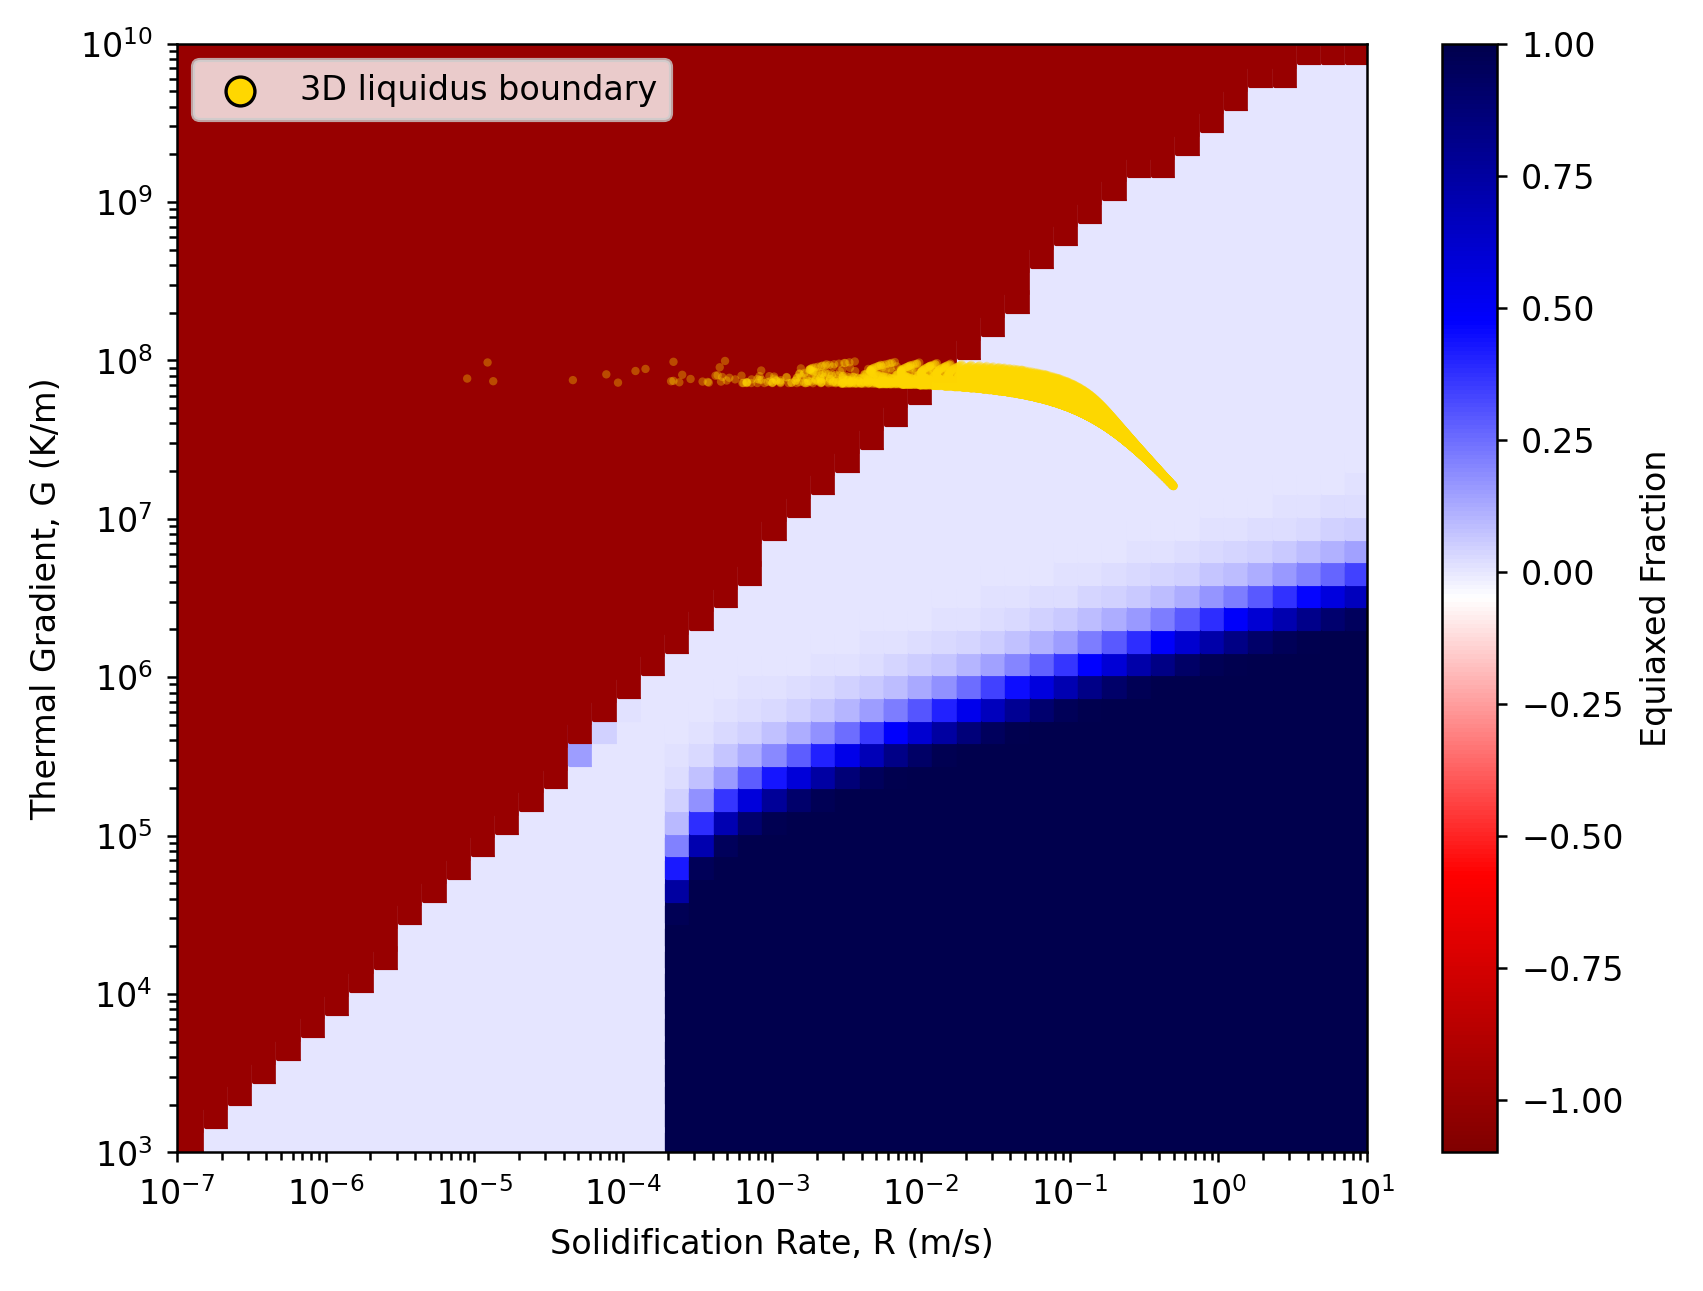
\includegraphics[width=\linewidth,height=0.58\textheight,keepaspectratio]{../beamer/figures/250_0.5/GR_map_overlayET_alloy0_250_0.5.png}
      \end{minipage}

      \vspace{0.25em}
      {\fontsize{15}{18}\selectfont GR Map calculated with Thermo-Calc CET Property Model with overlaid GR liquidus points for Hf$_2$Mo$_2$Ta$_{48}$W$_{48}$ (at.\%), $P = 250$ W and $V = 0.5$ m/s.}
    \end{column}
    \begin{column}{0.08\textwidth}
      \centering
      \vspace{0.25\textheight}
      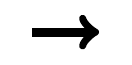
\begin{tikzpicture}
        \draw[->,line width=3.2pt,draw=black] (0,0) -- (0.85,0);
      \end{tikzpicture}
    \end{column}
    \begin{column}{0.45\textwidth}
      \centering
      \begin{minipage}[t][0.58\textheight][c]{\linewidth}
        \centering
        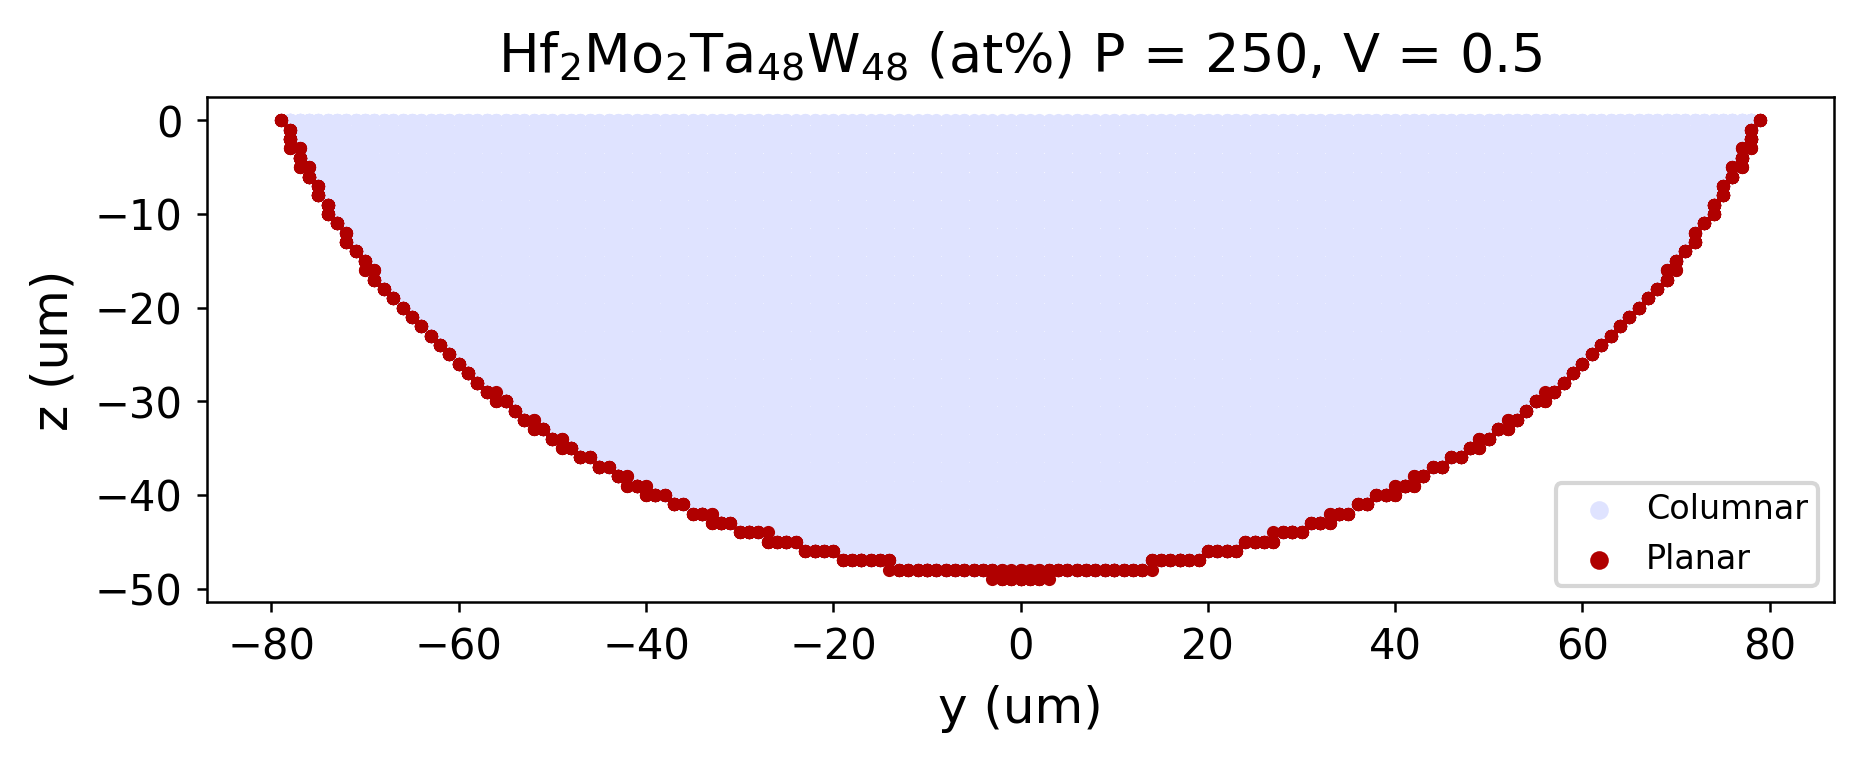
\includegraphics[width=\linewidth,height=0.58\textheight,keepaspectratio]{../beamer/figures/250_0.5/projected_microstructure_alloy0_250_0.5.png}
      \end{minipage}

      \vspace{0.25em}
      {\fontsize{15}{18}\selectfont Projected microstructure classification along the solidification front onto a $yz$ slice for Hf$_2$Mo$_2$Ta$_{48}$W$_{48}$ (at.\%), $P = 250$ W and $V = 0.5$ m/s.}
    \end{column}
  \end{columns}
\end{frame}

\begin{frame}{Thermo-Calc AM Module}
  \begin{columns}[T,onlytextwidth]
    \begin{column}{0.58\textwidth}
      \centering
      \begin{minipage}[t][0.67\textheight][c]{\linewidth}
        \centering
        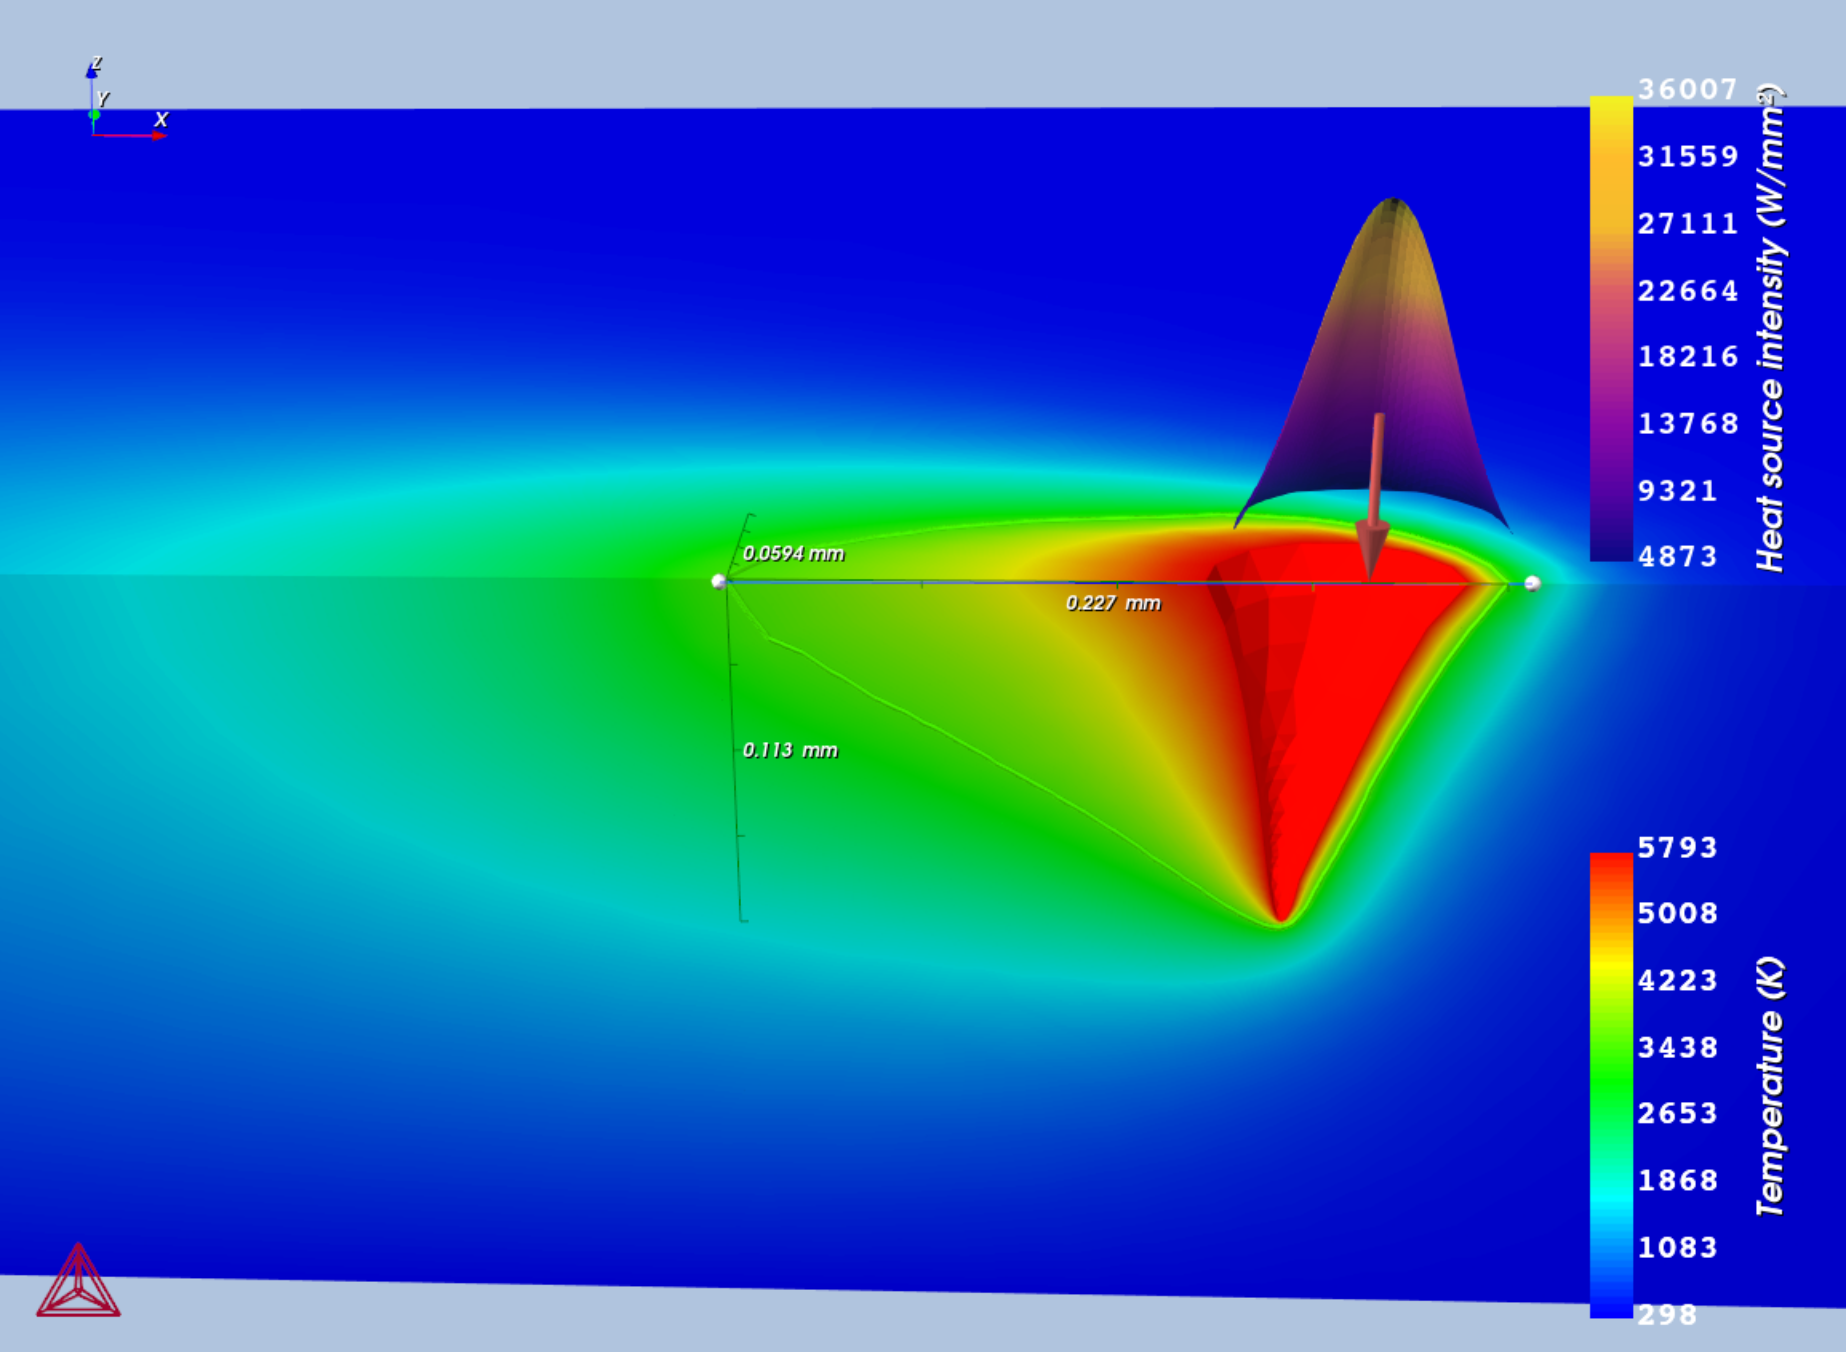
\includegraphics[width=\linewidth,height=0.67\textheight,keepaspectratio]{../beamer/figures/TCAM_alloy0_250_0.5.png}
      \end{minipage}

      \vspace{0.2em}
      {\fontsize{14}{17}\selectfont Steady-state TCAM simulation for Hf$_2$Mo$_2$Ta$_{48}$W$_{48}$ (at.\%), $P = 250$ W and $V = 0.5$ m/s.}
    \end{column}
    \begin{column}{0.40\textwidth}
      \begin{minipage}[t]{0.94\linewidth}
      \begin{block}{Higher-Fidelity Thermal Reference}
        \vspace{0.3em}
        \begin{itemize}
          \setlength{\itemsep}{0.35em}
          \item Integrates FEM for thermal conduction with CFD for melt-pool fluid flow.
          \item Composition-specific, temperature-dependent thermophysical properties.
          \item Captures Marangoni flow, keyholing, evaporation, radiation, and convection.
        \end{itemize}
        \vspace{0.3em}
      \end{block}

      \vspace{-0.25em}
      \begin{block}{Outputs Used in This Work}
        \vspace{0.3em}
        \begin{itemize}
          \setlength{\itemsep}{0.35em}
          \item 3D temperature field
          \item Melt-pool geometry
          \item Thermal gradient ($G$) and solidification rate ($R$) from ParaView post-processing
        \end{itemize}
        \vspace{0.3em}
      \end{block}

      \end{minipage}
    \end{column}
  \end{columns}
\end{frame}

\begin{frame}{TCAM Thermal Gradient and Solidification Rate}
  \begin{columns}[T,onlytextwidth]
    \begin{column}{0.45\textwidth}
      \centering
      \vspace{-1.35em}
      \begin{minipage}[t][0.72\textheight][c]{\linewidth}
        \centering
        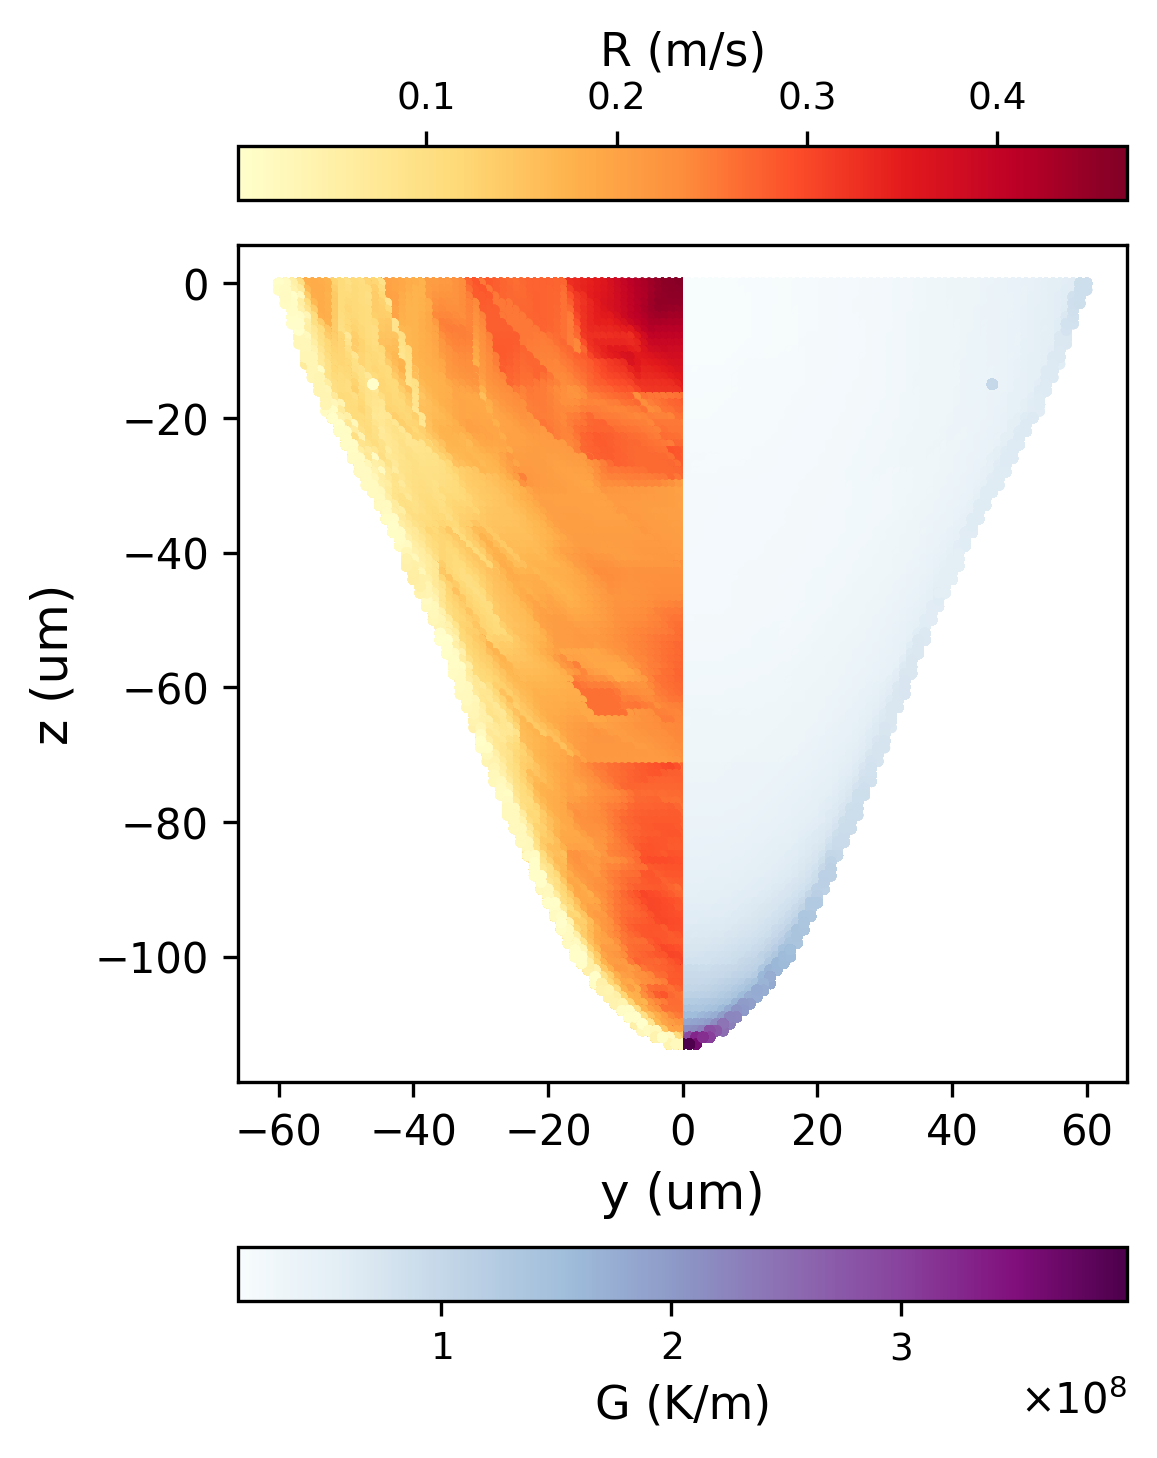
\includegraphics[width=\linewidth,height=0.72\textheight,keepaspectratio]{../beamer/figures/TCAM/TCAM_projected_GR_alloy0_250_0.5.png}
      \end{minipage}

      \vspace{0.25em}
      \hspace*{1.6em}\begin{minipage}{0.93\linewidth}
        {\fontsize{15}{18}\selectfont TCAM projection of $G$ and $R$ along the solidification front onto a $yz$ slice for Hf$_2$Mo$_2$Ta$_{48}$W$_{48}$ (at.\%), $P = 250$ W and $V = 0.5$ m/s.}
      \end{minipage}
    \end{column}
    \begin{column}{0.08\textwidth}
      \centering
      \vspace{0.25\textheight}
      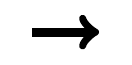
\begin{tikzpicture}
        \draw[->,line width=3.2pt,draw=black] (0,0) -- (0.85,0);
      \end{tikzpicture}
    \end{column}
    \begin{column}{0.45\textwidth}
      \centering
      \vspace{-1.35em}
      \begin{minipage}[t][0.72\textheight][c]{\linewidth}
        \centering
        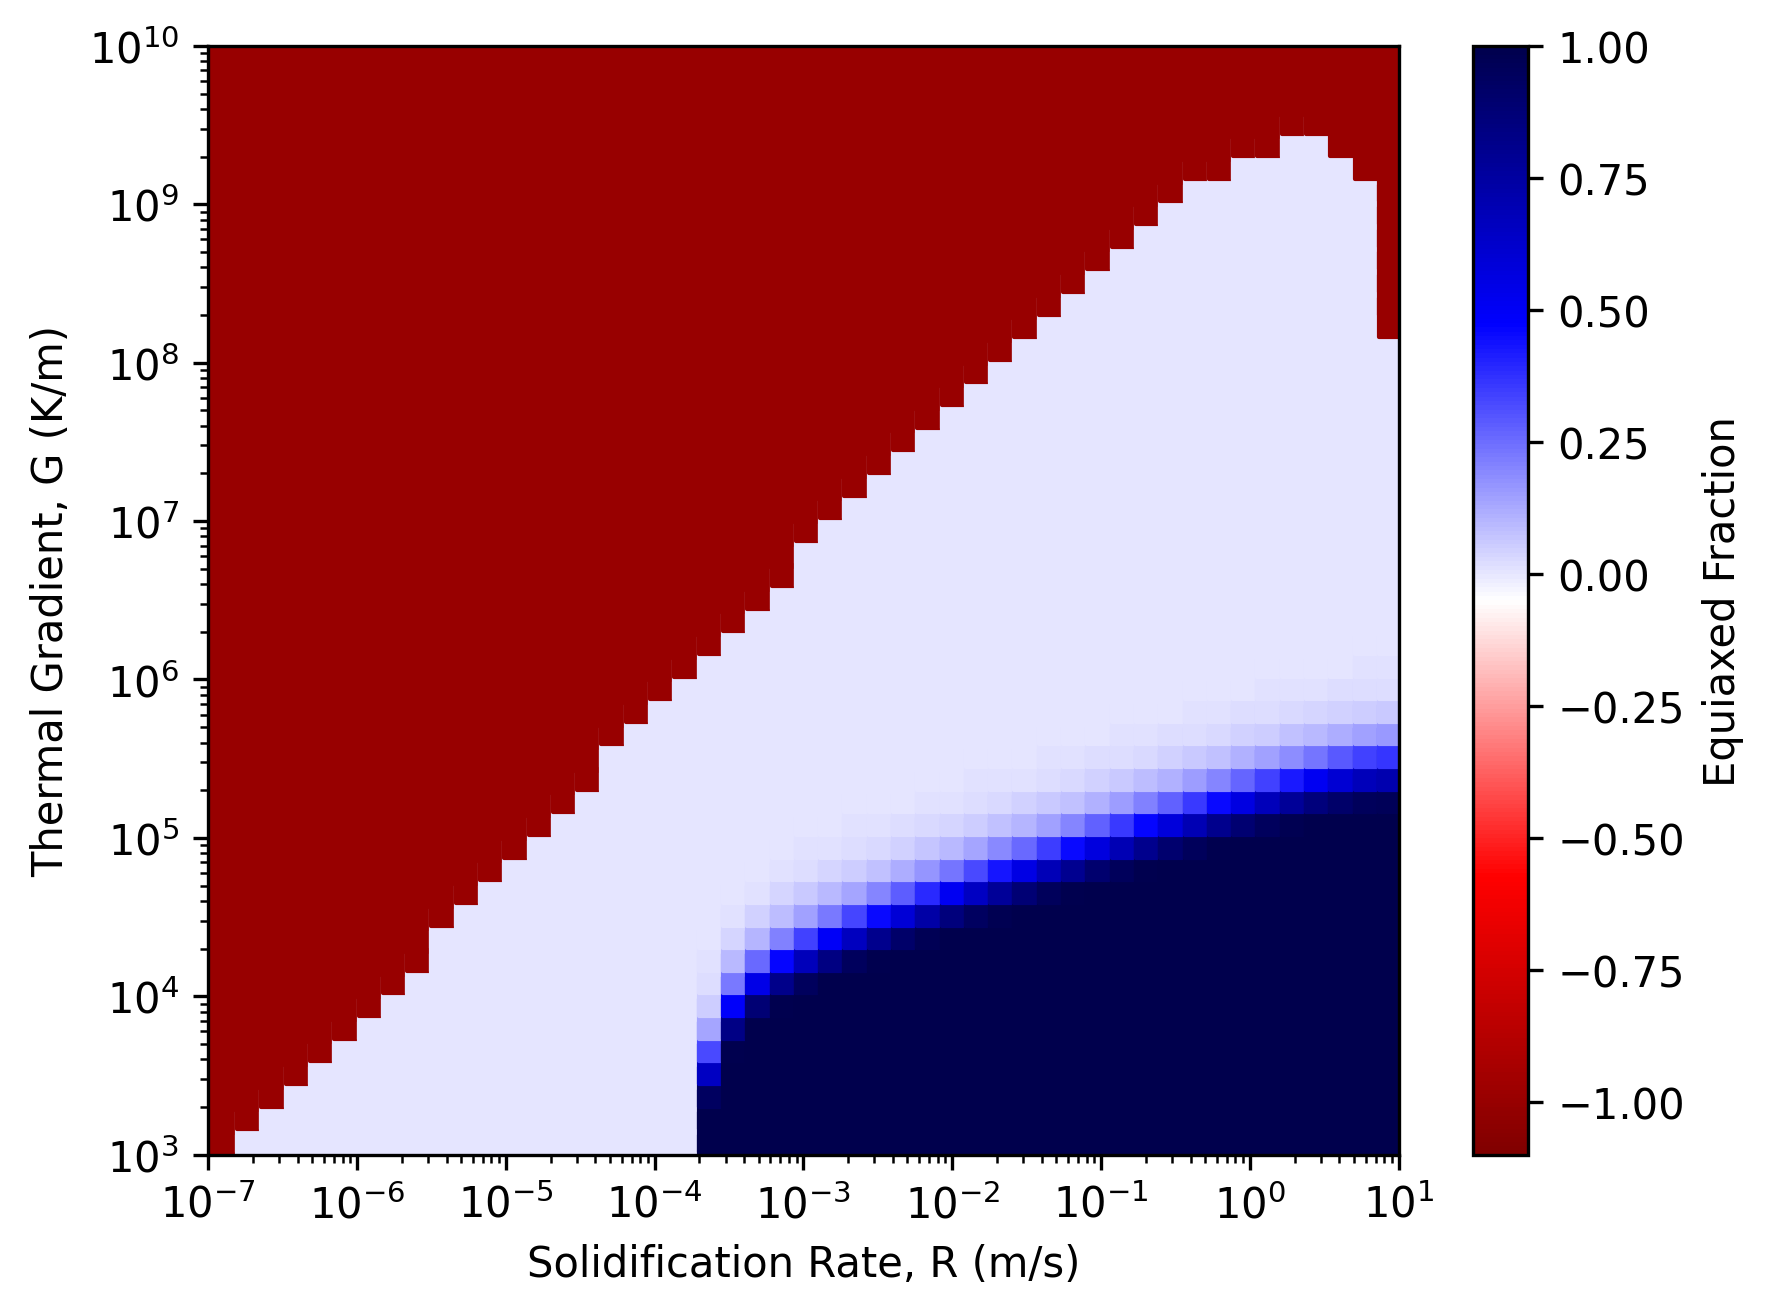
\includegraphics[width=\linewidth,height=0.58\textheight,keepaspectratio]{../beamer/figures/TCAM/GR_map_alloy0_250_0.5.png}
      \end{minipage}

      \vspace{0.25em}
      {\fontsize{15}{18}\selectfont GR Map calculated with the Thermo-Calc CET Property Model for Hf$_2$Mo$_2$Ta$_{48}$W$_{48}$ (at.\%), $P = 250$ W and $V = 0.5$ m/s.}
    \end{column}
  \end{columns}
\end{frame}

\begin{frame}{TCAM Microstructure Classification}
  \begin{columns}[T,onlytextwidth]
    \begin{column}{0.45\textwidth}
      \centering
      \begin{minipage}[t][0.65\textheight][c]{\linewidth}
        \centering
        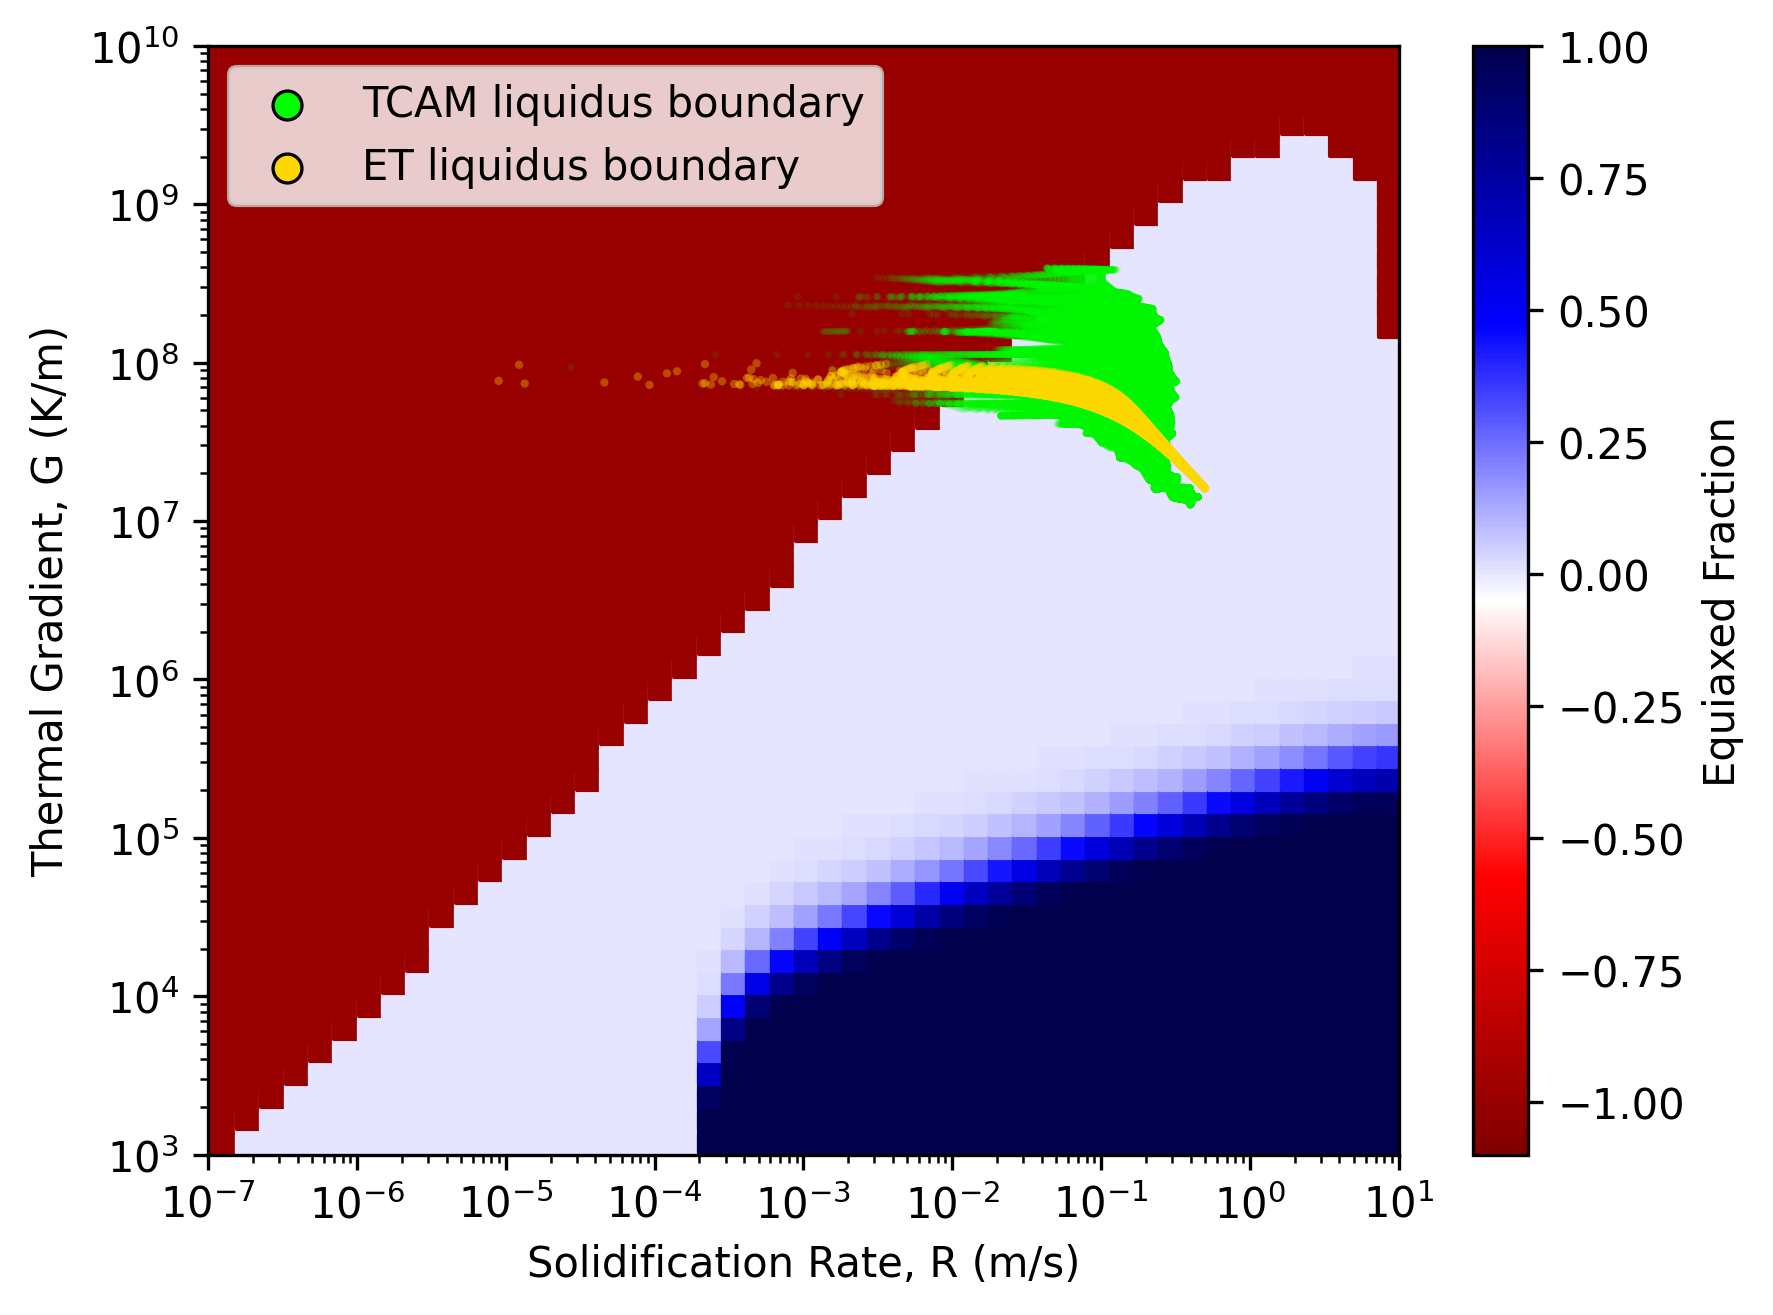
\includegraphics[width=\linewidth,height=0.58\textheight,keepaspectratio]{../beamer/figures/TCAM/GR_map_overlayET_TCAM_alloy0_250_0.png}
      \end{minipage}

      \vspace{0.25em}
      {\fontsize{15}{18}\selectfont GR map with TCAM and Eagar--Tsai liquidus-boundary conditions overlaid for Hf$_2$Mo$_2$Ta$_{48}$W$_{48}$ (at.\%), $P = 250$ W and $V = 0.5$ m/s.}
    \end{column}
    \begin{column}{0.08\textwidth}
      \centering
      \vspace{0.25\textheight}
      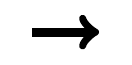
\begin{tikzpicture}
        \draw[->,line width=3.2pt,draw=black] (0,0) -- (0.85,0);
      \end{tikzpicture}
    \end{column}
    \begin{column}{0.45\textwidth}
      \centering
      \begin{minipage}[t][0.65\textheight][c]{\linewidth}
        \centering
        \hspace*{-0.8em}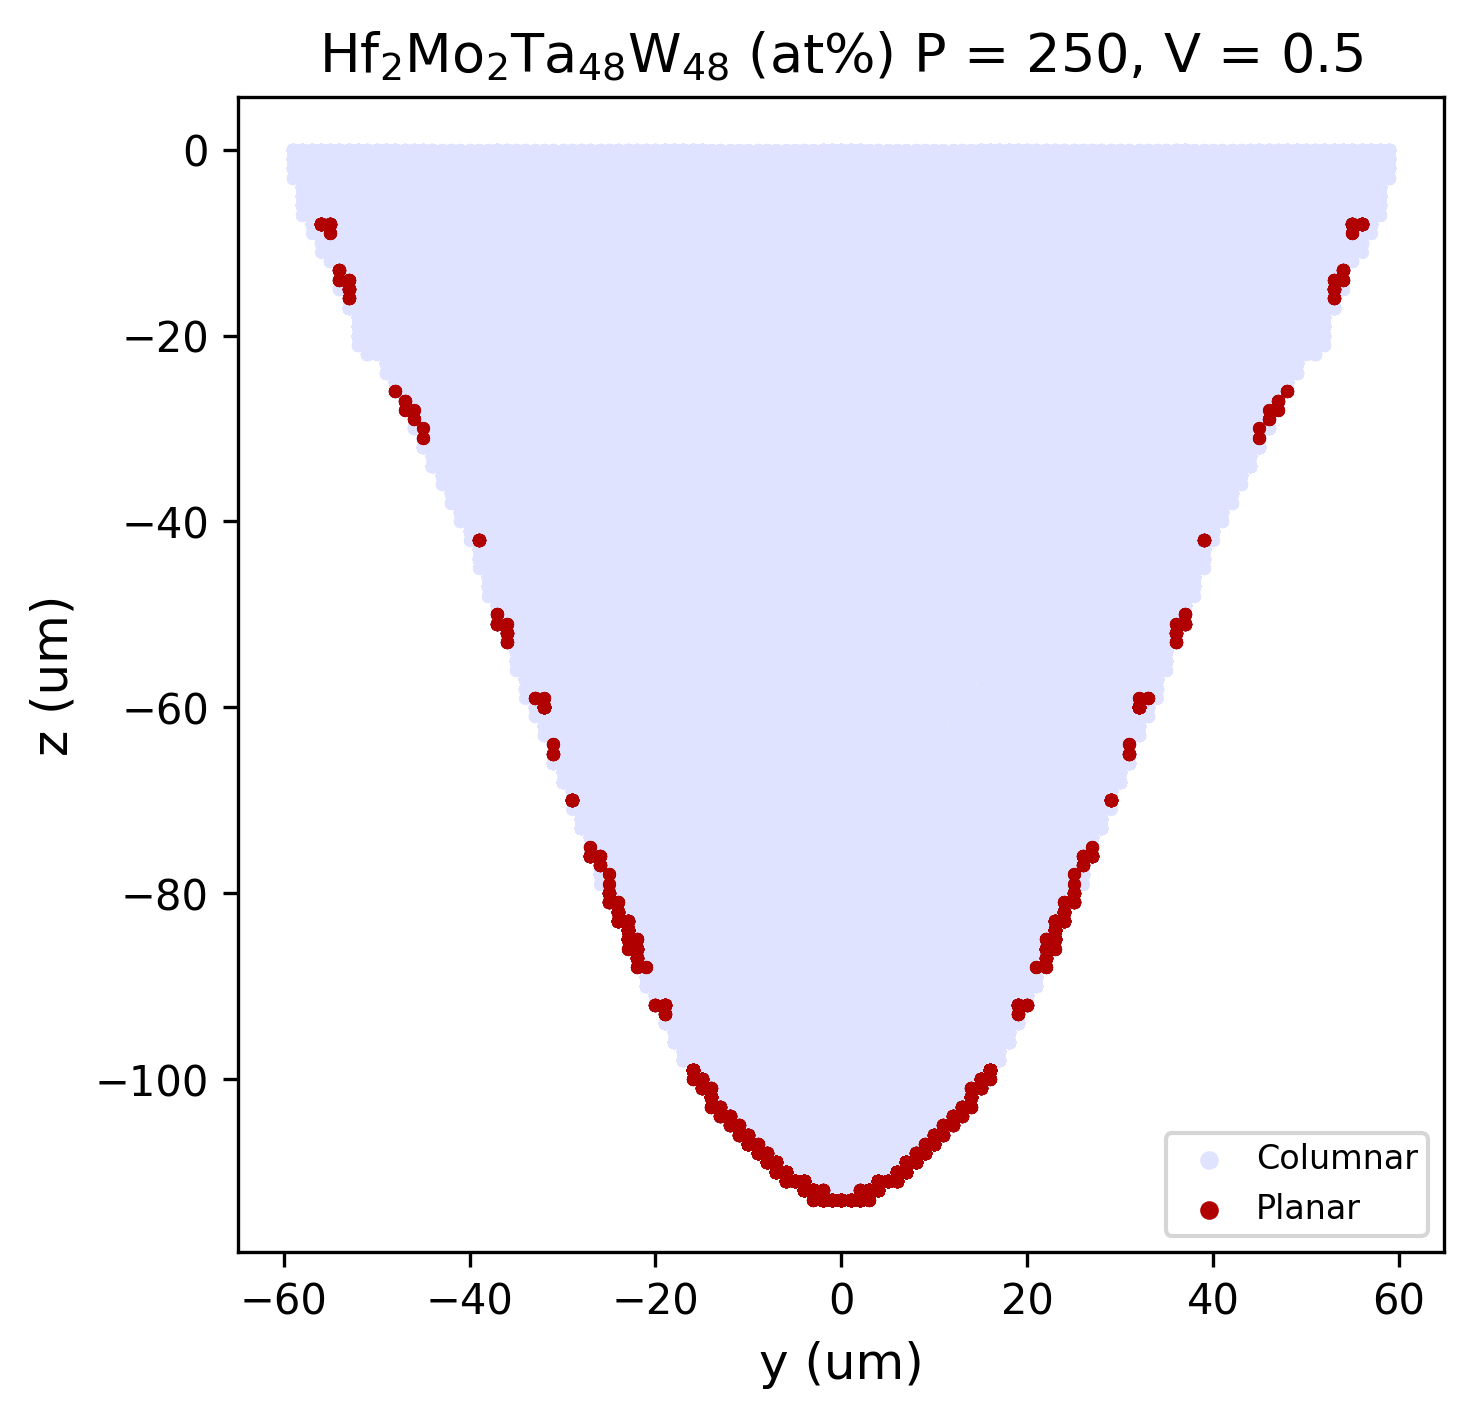
\includegraphics[width=\linewidth,height=0.65\textheight,keepaspectratio]{../beamer/figures/TCAM/TCAM_projected_microstructure_alloy0_250_0.5.png}
      \end{minipage}

      \vspace{0.25em}
      {\fontsize{15}{18}\selectfont TCAM-derived microstructure classification projected along the solidification front onto a $yz$ slice for the same alloy and process condition.}
    \end{column}
  \end{columns}
\end{frame}

\begin{frame}{ET vs.\ TCAM -- Melt Pool Comparison}
  \vspace{-1.0em}
  \hspace*{0.25cm}%
  \begin{minipage}{\textwidth}
  \begin{columns}[c,onlytextwidth]
    \begin{column}{0.28\textwidth}
      \raggedleft
      \raisebox{0.70cm}{%
        \hspace*{1.0cm}%
        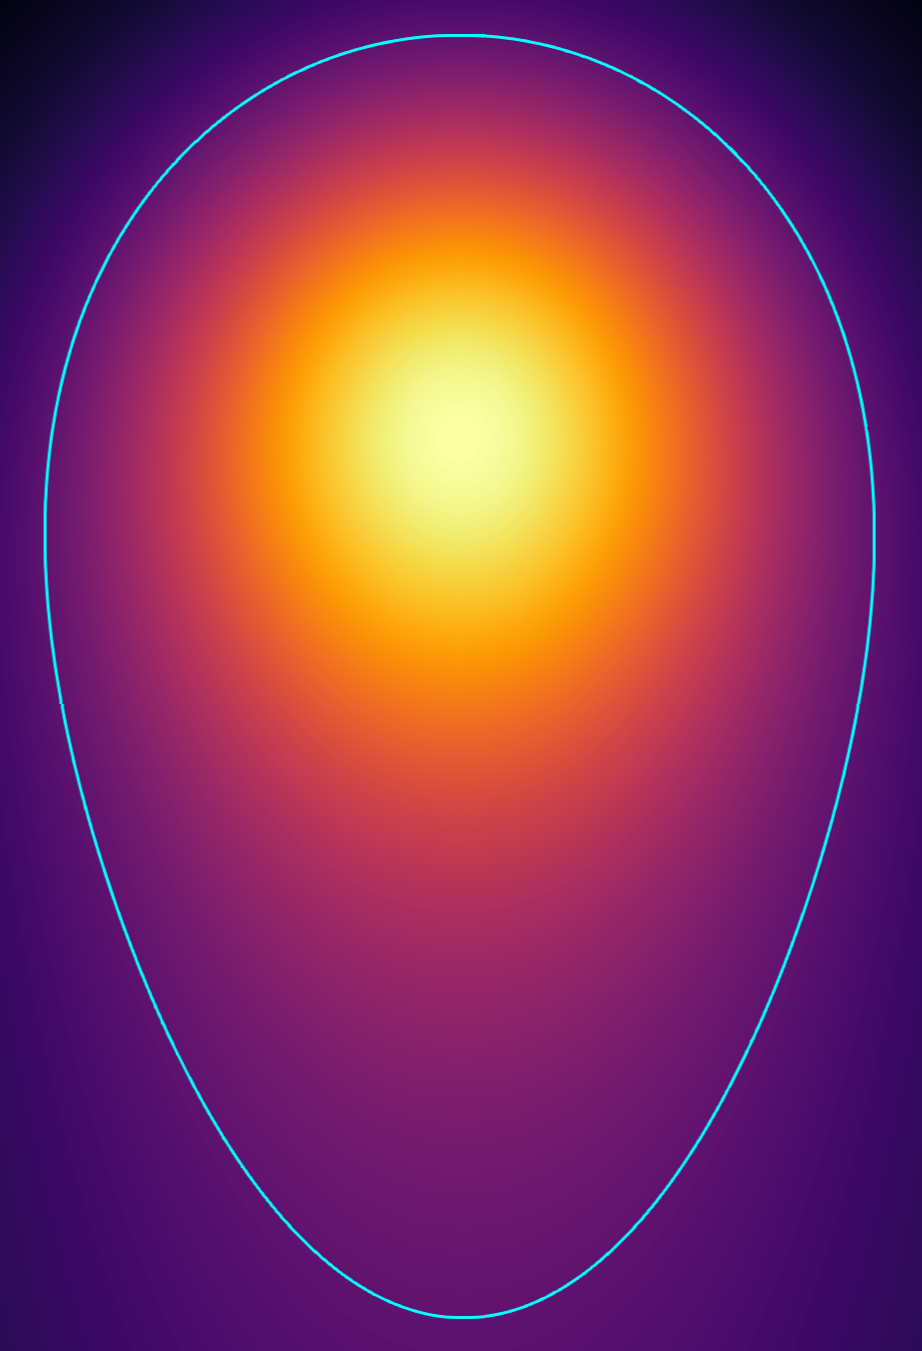
\includegraphics[
          height=0.715\textheight
        ]{../beamer/figures/et_melt_pool_vertical.png}%
      }
    \end{column}
    \begin{column}{0.46\textwidth}
      \centering
      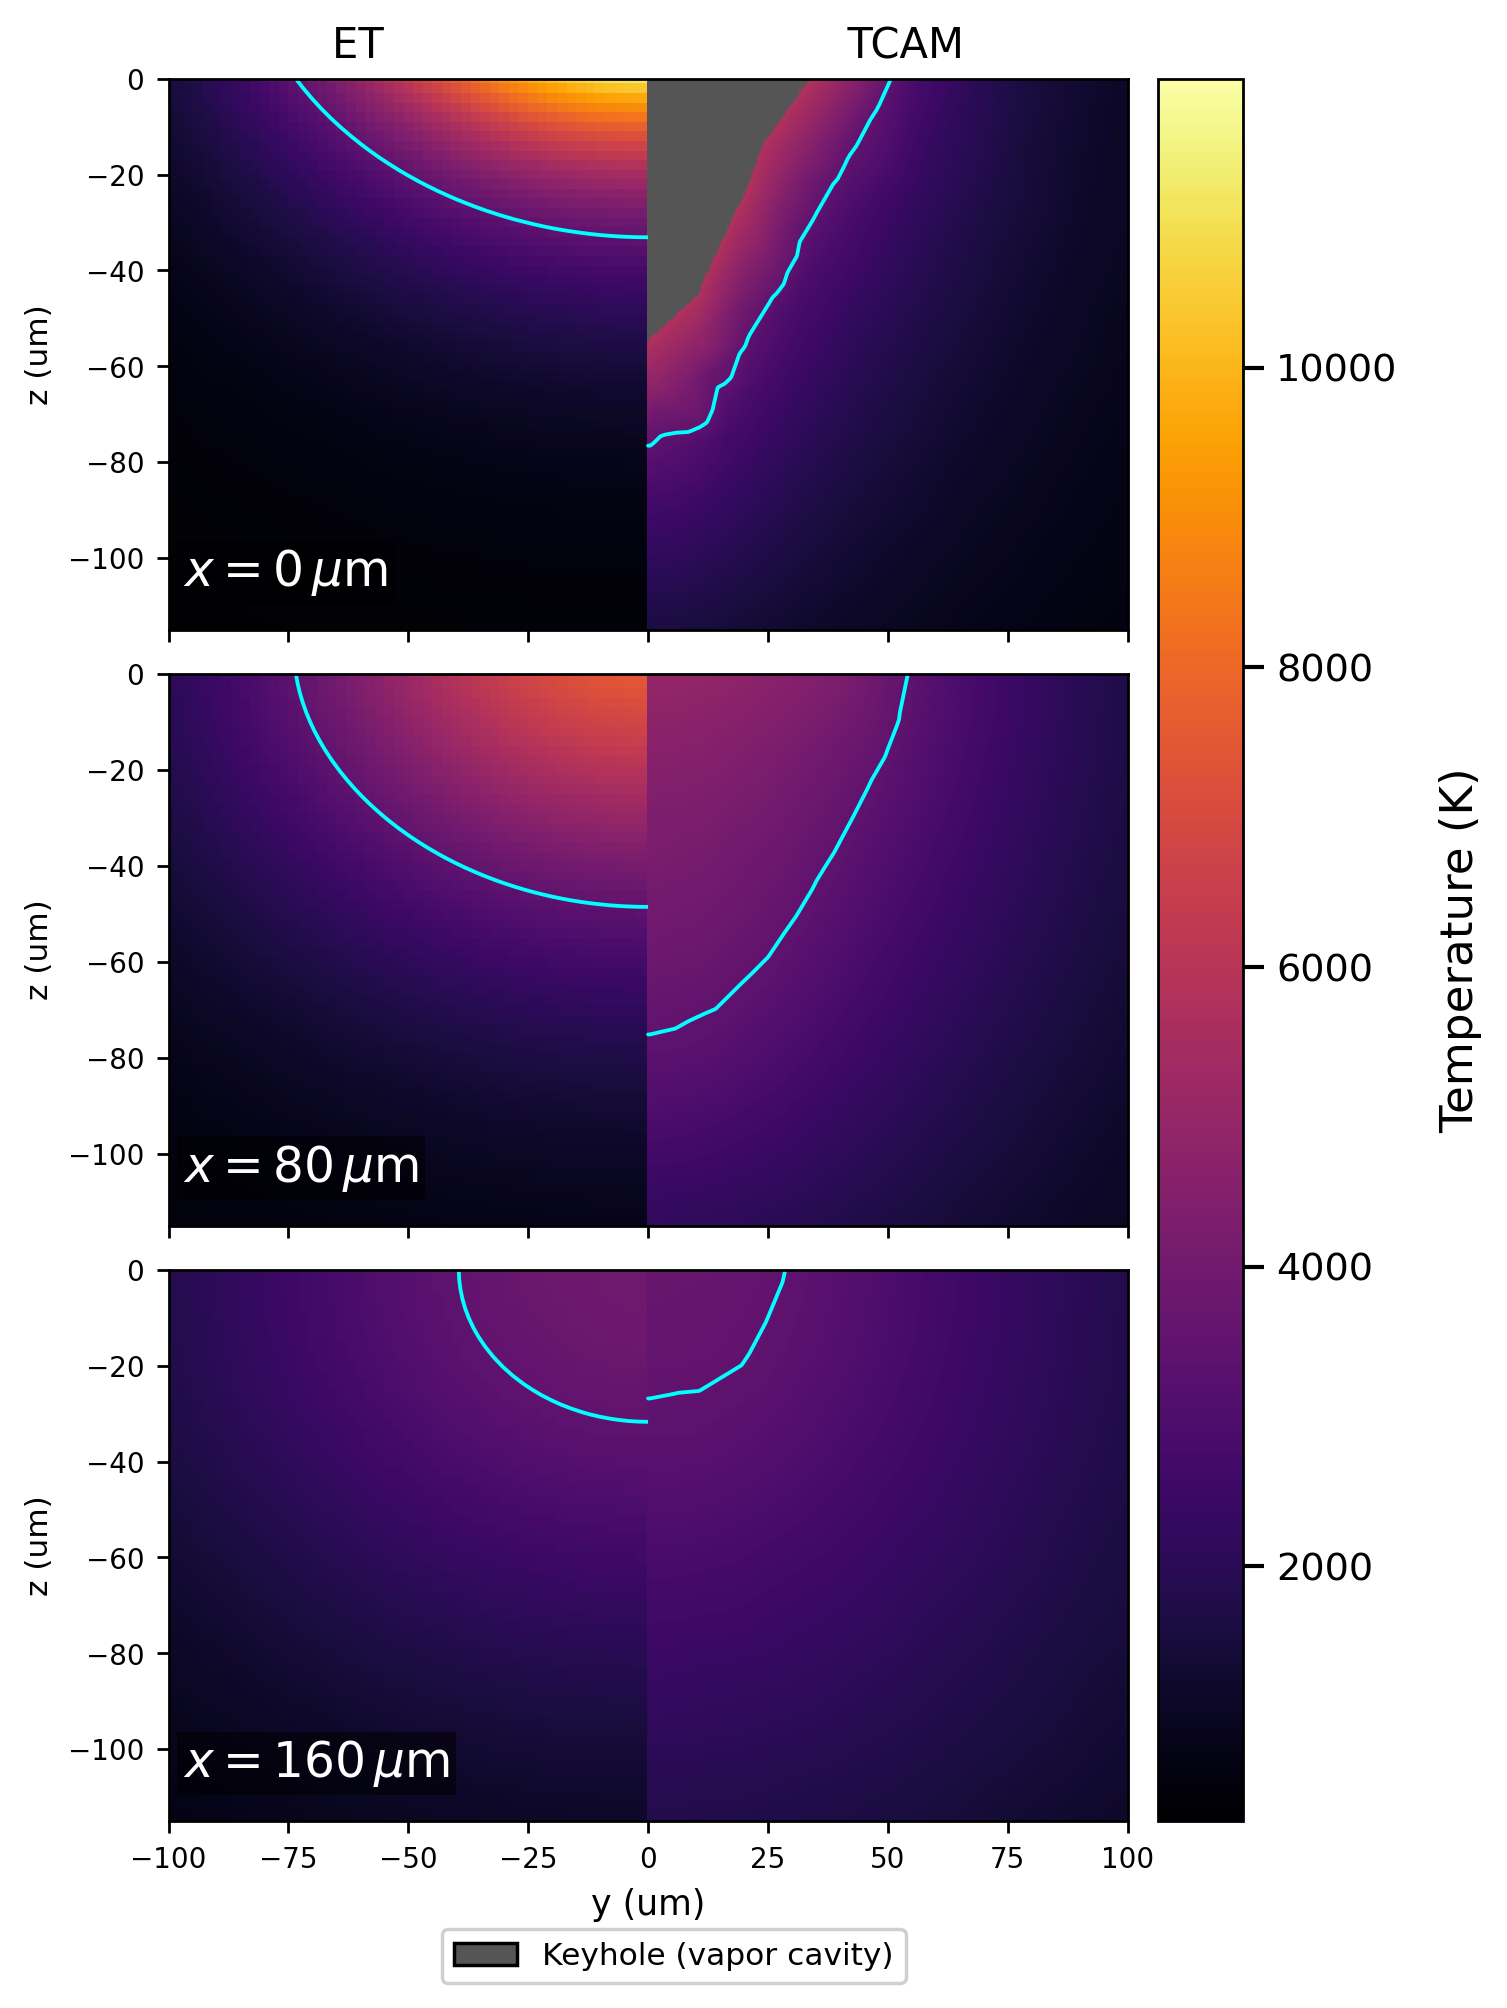
\includegraphics[
        width=\linewidth,
        height=0.82\textheight,
        keepaspectratio
      ]{../beamer/figures/TCAM/ET_TC_temp_yz_0_80_160um_inferno.png}
    \end{column}
    \begin{column}{0.23\textwidth}
      \raggedright
      \raisebox{0.70cm}{%
        \hspace*{-1.3cm}%
        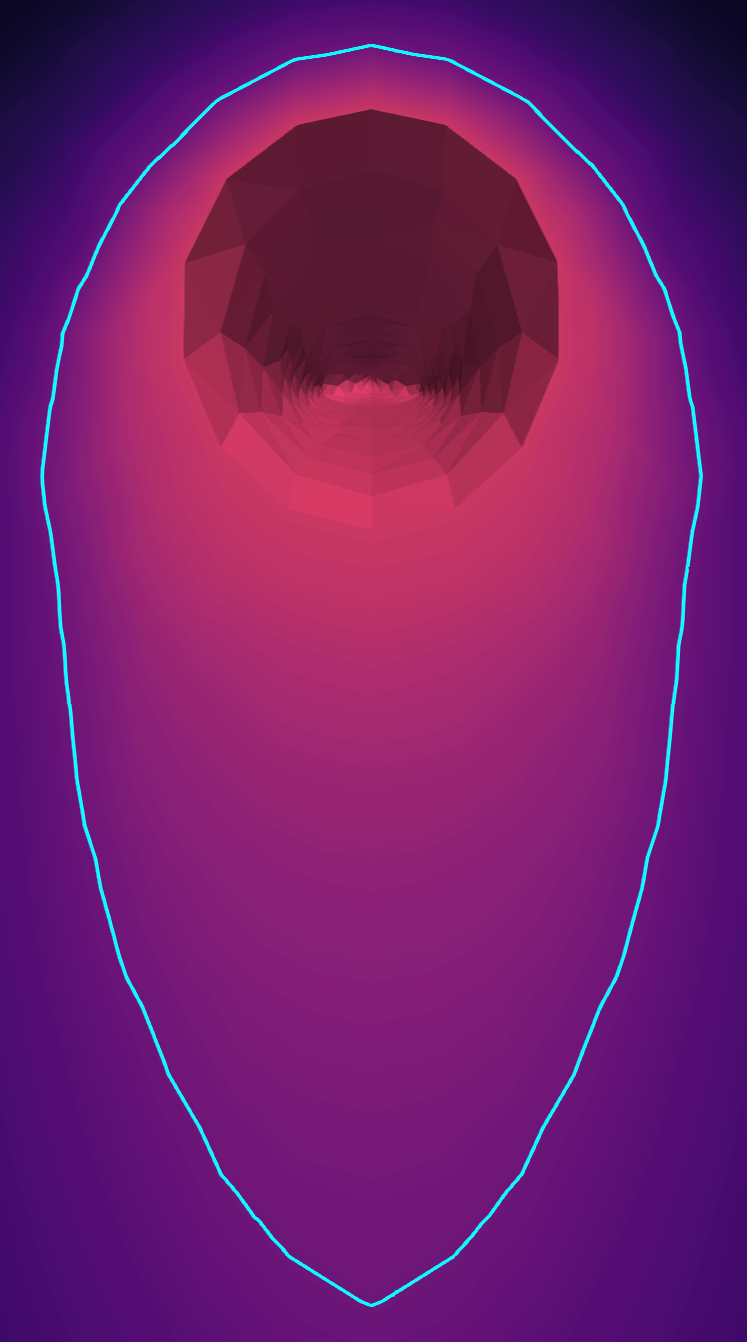
\includegraphics[
          height=0.715\textheight
        ]{../beamer/figures/tc_melt_pool_vertical.png}%
      }
    \end{column}
  \end{columns}
  \end{minipage}
\end{frame}

\begin{frame}{Bayesian Updating}
  \vspace{-0.85em}
  \setbeamerfont{block title}{size=\fontsize{19}{23}\selectfont,series=\bfseries}
  \setbeamerfont{block body}{size=\fontsize{18}{22}\selectfont}
  \begin{columns}[T,onlytextwidth]
    \begin{column}{0.40\textwidth}
      \hspace*{1.30cm}%
      \begin{minipage}[t]{\dimexpr\linewidth-1.30cm\relax}
        \raggedright
        \vspace*{1.00cm}
        {\fontsize{23}{27}\selectfont
        \textcolor{sffblue}{\textbf{Physics-informed correction}}\par}

        \vspace{0.65em}
        {\fontsize{20}{25}\selectfont
        Eagar--Tsai provides a fast, structured prior across the full melt-pool
        domain.

        \vspace{0.8em}
        Targeted TCAM simulations act as the high-fidelity ``ground truth'' that
        teaches the model where and why the prior is wrong.

        \vspace{0.8em}
        The correction is learned without discarding the underlying ET physics.\par}
      \end{minipage}
    \end{column}

    \begin{column}{0.56\textwidth}
      \hfill
      \begin{minipage}{0.82\linewidth}
        \begin{block}{1. ET Physics Prior}
          \centering
          Predict temperature rapidly throughout the full melt-pool domain for
          a spatial location $\mathbf{s}$ and process condition $\theta$.

          \vspace{0.15em}
          {\fontsize{20}{24}\selectfont
          $T_{\mathrm{ET}}(\mathbf{s},\theta)$}
        \end{block}
      \end{minipage}
      \hfill\strut\par

      \vspace{-0.12em}
      \centering
      \begin{tikzpicture}
        \draw[-{Stealth[length=3.2mm]},line width=2.2pt,sffblue]
          (0,0.18) -- (0,-0.48);
      \end{tikzpicture}
      \vspace{-0.25em}

      \hfill
      \begin{minipage}{0.82\linewidth}
        \begin{block}{2. TCAM Training Evidence}
          \centering
          Sample high-fidelity temperatures at selected spatial locations and
          process conditions, then match them to the ET field.

          \vspace{0.15em}
          {\fontsize{20}{24}\selectfont
          $T_{\mathrm{TCAM}}(\mathbf{s},\theta)$}
        \end{block}
      \end{minipage}
      \hfill\strut\par

      \vspace{-0.12em}
      \centering
      \begin{tikzpicture}
        \draw[-{Stealth[length=3.2mm]},line width=2.2pt,sffblue]
          (0,0.18) -- (0,-0.48);
      \end{tikzpicture}
      \vspace{-0.25em}

      \hfill
      \begin{minipage}{0.82\linewidth}
        \begin{block}{3. GPR Discrepancy Model}
          \centering
          Train the Gaussian process on the structured error rather than
          replacing the physics model with a purely data-driven predictor.

          \vspace{0.15em}
          {\fontsize{20}{24}\selectfont
          $\Delta T=T_{\mathrm{TCAM}}-T_{\mathrm{ET}}$}
        \end{block}
      \end{minipage}
      \hfill\strut\par
    \end{column}
  \end{columns}
\end{frame}

\begin{frame}{Bayesian-Updated ET Model}
  \vspace{-0.45em}
  \begin{block}{Posterior Temperature Field}
    \begin{columns}[c,onlytextwidth]
      \begin{column}{0.56\textwidth}
        ET supplies the physics-based baseline; the GPR posterior mean supplies
        the TCAM-informed correction.
      \end{column}
      \begin{column}{0.40\textwidth}
        \centering
        {\fontsize{22}{27}\selectfont
        $T_{\mathrm{updated}}=T_{\mathrm{ET}}+\mu_{\Delta T}$}
      \end{column}
    \end{columns}
  \end{block}

  \vspace{0.45em}
  \begin{columns}[T,onlytextwidth]
    \begin{column}{0.32\textwidth}
      \begin{block}{Spatial Correction}
        Learns where and by how much ET over- or under-predicts temperature
        throughout the melt pool.
      \end{block}
    \end{column}
    \begin{column}{0.32\textwidth}
      \begin{block}{Process Sensitivity}
        Across multiple TCAM conditions, learned feature length scales and
        sensitivity reveal how $P$, $v$, $d_b$, and $A$ affect the thermal field
        and melt-pool geometry.
      \end{block}
    \end{column}
    \begin{column}{0.32\textwidth}
      \begin{block}{Predictive Uncertainty}
        The posterior variance shows where the correction is trusted and where
        another TCAM training point would add the most information.
      \end{block}
    \end{column}
  \end{columns}

  \vspace{0.55em}
  {\fontsize{16}{20}\selectfont\centering
  The updated temperature field can then be propagated to melt-pool geometry,
  $G$--$R$ conditions, and microstructure classification.\par}
\end{frame}

\begin{frame}{Closing}
  \begin{block}{Takeaway}
    End with the decision, ask, or technical conclusion you want the audience to remember.
  \end{block}
  \vspace{0.5em}
  \begin{itemize}
    \item \deliverable{Deliverable}: Name the concrete output.
    \item \risk{Primary risk}: Name the hardest unresolved issue.
    \item \stage{Immediate next step}: Name the action that starts now.
  \end{itemize}
\end{frame}

\end{document}
